\documentclass{article} % For LaTeX2e
\usepackage{nips14submit_e,times}
\usepackage{hyperref}
\usepackage{url}
\usepackage{amsfonts}
\usepackage{amssymb,amsmath}
\usepackage{amsthm}
\usepackage{graphicx}
\usepackage{color}
%\usepackage[usenames,dvipsnames]{xcolor}
\usepackage{caption}
\usepackage{subcaption}
\usepackage{placeins}
\usepackage{enumitem}
\usepackage{wrapfig}
%\documentstyle[nips14submit_09,times,art10]{article} % For LaTeX 2.09

\newtheorem{definition}{Definition}
\newtheorem{lemma}{Lemma}
\newtheorem{Theorem}{Theorem}
\newtheorem{example}{Example}
\newtheorem{statement}{Statement}
\newtheorem{corollary}{Corollary}
\newtheorem{proposition}{Proposition}
\usepackage{mathtools}

\newcommand{\indep}{\rotatebox[origin=c]{90}{$\models$}}
 \newcommand{\ev}{\mathcal{E}}

\DeclarePairedDelimiter\norm{\lVert}{\rVert}
%\title{Wild and Degenerate - Bootstrap For Kernel Methods}
\title{A Wild Bootstrap for Degenerate Kernel Tests}

\author{
David S.~Hippocampus\thanks{ Use footnote for providing further information
about author (webpage, alternative address)---\emph{not} for acknowledging
funding agencies.} \\
Department of Computer Science\\
Cranberry-Lemon University\\
Pittsburgh, PA 15213 \\
\texttt{hippo@cs.cranberry-lemon.edu} \\
\And
Coauthor \\
Affiliation \\
Address \\
\texttt{email} \\
\AND
Coauthor \\
Affiliation \\
Address \\
\texttt{email} \\
\And
Coauthor \\
Affiliation \\
Address \\
\texttt{email} \\
\And
Coauthor \\
Affiliation \\
Address \\
\texttt{email} \\
(if needed)\\
}

% The \author macro works with any number of authors. There are two commands
% used to separate the names and addresses of multiple authors: \And and \AND.
%
% Using \And between authors leaves it to \LaTeX{} to determine where to break
% the lines. Using \AND forces a linebreak at that point. So, if \LaTeX{}
% puts 3 of 4 authors names on the first line, and the last on the second
% line, try using \AND instead of \And before the third author name.

\newcommand{\fix}{\marginpar{FIX}}
\newcommand{\new}{\marginpar{NEW}}
%\nipsfinalcopy % Uncomment for camera-ready version
\newcommand{\Hk}{\ensuremath{\mathcal{H}_k}}%
\begin{document}


\maketitle

\begin{abstract}
%Wild Bootstrap For Kernel Methods is awesome.

  A wild bootstrap method for nonparametric hypothesis
  tests based on kernel distribution embeddings is proposed. This
  bootstrap method is used to construct provably consistent tests that apply to random
  processes, for which the naive permutation-based bootstrap
  fails. It applies to a large group of kernel tests
  based on V-statistics, which are degenerate under the null
  hypothesis, and non-degenerate elsewhere. To illustrate this
  approach, we construct a two-sample test, an instantaneous independence
  test and a multiple lag independence test for time series.  In experiments, the wild
  bootstrap gives strong performance on synthetic examples, on audio
  data, and in performance benchmarking for the Gibbs sampler.


%In experiments, the tests constructed using wild bootstrap method give strong performance on synthetic examples, on audio data, and in  performance benchmarking for the Gibbs sampler, outperforming some of existing methods.
\iffalse
A general-purpose nonparametric testing procedure is proposed
 in the case where the variables
being tested are time series, 
based on kernel distribution embeddings. The approach makes use of a wild
bootstrap procedure to obtain a test threshold, yielding
a test with the correct Type I error, and a Type II error approaching 
zero, as the number of samples increases.  The wild bootstrap 
 applies to all kernel tests based on V-statistics, which
are degenerate under the null hypothesis, and non-degenerate elsewhere 
(the present work treats both two-sample and independence testing).
Further, it is possible to test dependence between time series which might
occur  over a range of time lags, rather than at a given fixed lag.
In experiments, the wild bootstrap gives strong performance
on synthetic examples, on audio data, 
and in  performance benchmarking for the Gibbs sampler.
\fi

\end{abstract}


%I assume that after reading a section in the introduction a reader will have basic understanding of what a wild bootstrap is and why is it useful. He will be also informed about the following contributions
%\begin{itemize}
%\item Wild Bootstrap For Higher Order $V$-statistics - application to HSIC and three variables interaction
%\item Test for 'total' independence of two time series as KCSD and experimental results
%\item (?) Outline of how two sample can be used to test  MCMC convergence and experimental premise that it is feasible.    
%\end{itemize}  

\vspace{-4mm}
\section{Introduction}
\vspace{-3mm}


Statistical tests based on distribution embeddings into reproducing kernel Hilbert spaces have been applied in many contexts,  including two sample testing \cite{HarBacMou08,gretton2012kernel,SugSuzItoKanetal11}, tests of independence \cite{gretton_kernel_2008,ZhaPetJanSch11,besserve_statistical_2013}, tests of conditional independence  \cite{fukumizu2007kernel,ZhaPetJanSch11}, and tests for higher order (Lancaster) interactions \cite{sejdinovic2013kernel}. %
% AG: if we are looking to save space in the bibliography we can cut the three references below. However it is important to have the references above, since they are more directly related to the theory-minded paper we're writing.
%Although relatively new, these tests have already influenced research beyond machine learning and proved to be useful tools in domains such as genomics \cite{Schweikert2013}, steganography \cite{Solanki2008} and econometrics \cite{zaremba2014measures}.       
For these tests,  consistency is guaranteed if and only if the observations are independent and identically distributed. 
Much real-world data fails to satisfy the i.i.d. assumption: audio signals, EEG recordings, text documents, financial time series, and samples obtained when running Markov Chain Monte Carlo, all show  significant temporal dependence patterns.  

The asymptotic behaviour of kernel test statistics becomes quite different when temporal dependencies exist within
the samples.
In recent work on independence testing using the Hilbert-Schmidt Independence
Criterion (HSIC) \cite{chwialkowski2014kernel}, the asymptotic distribution of the statistic under the null hypothesis is obtained for a pair of independent time series, which satisfy an absolute regularity or a $\phi$-mixing assumption.
In this case, the null distribution is shown to be an infinite weighted sum of {\em dependent} $\chi^2$-variables,
as opposed to the sum of \emph{independent} $\chi^2$-variables obtained in the i.i.d. setting \cite{gretton_kernel_2008}.
The difference in the asymptotic null distributions has important implications in practice:
under the i.i.d. assumption, an empirical estimate of the null distribution can be obtained by
repeatedly permuting the time indices of one of the signals. This breaks
the temporal dependence within the permuted signal, which causes the test to return an elevated
number of false positives, when used for testing time series. To address this problem, an alternative estimate of the null distribution
is proposed in \cite{chwialkowski2014kernel}, where the null distribution is simulated by repeatedly
{\em shifting} one
signal relative to the other. This preserves the temporal structure within each signal, while breaking the cross-signal
dependence.

A serious limitation of the shift procedure in \cite{chwialkowski2014kernel} is that it is specific
to the problem of independence testing: there is no obvious way to generalise it to  other
testing contexts. For instance, we might have two time series, with the goal of comparing
their marginal distributions - this is a generalization of the two-sample setting to which the shift
approach does not apply.

We note, however, that many kernel tests have a test statistic with a particular structure:  the Maximum Mean Discrepancy (MMD), HSIC, and the Lancaster interaction statistic,
each have empirical estimates which can be cast as normalized $V$-statistics,
$\frac{1} {n^m-1} \sum_{1\leq i_1,...,i_m \leq n} h(Z_{i_1},...,Z_{i_m})$,
where $Z_{i_1},...,Z_{i_m}$ are samples from a random process at the time points $\{i_1,\ldots,i_m\}$. We show that
a method of external randomization known as the {\em wild bootstrap} may be applied  \cite{leucht_dependent_2013,Shao2010} to simulate from the null distribution.
In brief, the arguments of the above sum are repeatedly multiplied by random, user-defined time series. For a test of level
$\alpha$, the $1-\alpha$ quantile of the empirical distribution obtained using these perturbed statistics serves as the test threshold. This approach has the important advantage over \cite{chwialkowski2014kernel} that it may be applied to {\em all} kernel-based tests for which V-statistics are employed, and not just in the independence setting.

The main result of this paper is to show that the wild bootstrap procedure yields consistent tests for time series, i.e., tests based on the wild bootstrap  have a Type I error rate (of wrongly rejecting the null hypothesis) approaching the design parameter $\alpha$, and a Type II error (of wrongly accepting the null) approaching zero, as the number of samples increases. We use this result to construct a two-sample test using MMD, and an independence test using HSIC. The latter procedure is applied both to testing for instantaneous independence, and to testing for independence across multiple time lags, for which the earlier shift procedure of \cite{chwialkowski2014kernel} cannot be applied.

%DS: commented as we have the same point in the next paragraph...Out test against long range dependence is demonstrated to have an improved power in comparison to the related test by \cite{besserve_statistical_2013}.

%% AG: I moved the detailed MCMC discussion to the MCMC section

%Further, we construct a test of time series dependence similar to one proposed by \cite{besserve_statistical_2013} showing improvements in terms of detection errors.            

%Simultaneous testing for dependence of two time series across multiple time lags is also of interest, since it may not be a priori known at what lag the dependence occurs \cite{besserve_statistical_2013}. In this case, the shift procedure of \cite{chwialkowski2014kernel} can be problematic, as certain shifts may increase dependence between the time series, and it cannot be known in advance which shifts these will be. By contrast, the wild bootstrap can be used straightforwardly in this circumstance, and outperforms \cite{besserve_statistical_2013} in experiments.

We begin our presentation in Section \ref{sec:background}, with a review of the $\tau$-mixing assumption required of the time series, as well as of   V-statistics (of which MMD and HSIC are instances). We also introduce the form taken by the wild bootstrap. In Section \ref{sec:main}, we establish a general consistency result for the wild bootstrap procedure on V-statistics, which we apply to MMD and to HSIC in Section \ref{sec:mmd_hsic}. Finally, in Section \ref{sec:Experiments}, we present a number of empirical comparisons: in the two sample case, we test for differences in audio signals with the same underlying pitch, and present a performance diagnostic for the output of a Gibbs sampler; in the independence case, we test for independence of two time series sharing a common variance (a characteristic of econometric models), and compare against the test of \cite{besserve_statistical_2013} in the case where dependence may occur at multiple, potentially unknown lags. Our tests outperform both the naive approach which neglects the dependence structure within the samples, and the approach of \cite{besserve_statistical_2013}, when testing across multiple lags.

\vspace{-2mm}
\section{Background}\label{sec:background}
\vspace{-2mm}
The main results of the paper are based around two concepts: $\tau$-mixing \cite{dedecker2007weak}, which describes the dependence within the time series, and  $V$-statistics \cite{serfling80}, which constitute our test statistics. In this section, we review these topics, and introduce the concept of wild bootstrapped V-statistics, which will be the key ingredient in our test construction.

\paragraph{$\tau$-mixing.} The notion of $\tau$-mixing is used to characterise weak dependence. It is a less restrictive alternative to classical mixing coefficients, and is covered in depth in \cite{dedecker2007weak}. Let $\{Z_t,\mathcal{F}_t\}_{t \in \mathbb{N}}$  be a stationary sequence of integrable random variables, defined on a probability space $\Omega$ with a probability measure $P$ and a natural filtration $\mathcal{F}_t$. The process  is called $\tau$-dependent if 
\begin{align*}
\tau(r) &= \sup_{l \in \mathbb{N}} \frac 1 l \sup_{ r \leq i_1 \leq ... \leq i_l} \tau( \mathcal F_0,(Z_{i_1},...,Z_{i_l}) )  \overset{r \to \infty}{=} 0 \text{ , where} \\
\tau(\mathcal{M},X) &=  \ev \left( \sup_{g \in \Lambda} \left| \int g(t) P_{X|\mathcal{M}}(dt) - \int g(t) P_X(dt) \right| \right)
\end{align*}
and $\Lambda$ is the set of all one-Lipschitz continuous real-valued functions on the domain of $X$. $\tau(\mathcal M,X)$ can be interpreted as the minimal $L_1$ distance between $X$ and $X^*$ such that $X \overset{d}{=}X^*$ and $X^*$ is independent of $\mathcal M \subset \mathcal F$. Furthermore, if $\mathcal F$ is rich enough, this $X^*$ can be constructed (see Proposition \ref{prop:Coupling} in the Appendix).
  

\paragraph{V-statistics.} The test statistics considered in this paper are always $V$-statistics. Given the observations $Z=\left\{Z_t\right\}_{t=1}^n$, a $V$-statistic of a symmetric function $h$ taking $m$ arguments is given by 
\begin{equation}
\label{def:Vstat}
V(h,Z) = \frac{1}{n^m} \sum_{(i_1,...,i_m) \in N^m} h(Z_{i_1},...,Z_{i_m}),
\end{equation}
where $N^m$ is a Cartesian power of a set $N= \{1,...,n\}$. For simplicity, we will often drop the second argument and write simply $V(h)$. 
%DS: commented as it does not appear anywhere in the main text...We will  denote the tuple $(i_1,...,i_m)$ by $i$.
%i.e. $\sum_{i \in N^m} f(\cdot) \equiv \sum_{(i_1,...,i_m) \in N^m} f()$. 

We will refer to the function $h$ as to the \emph{core} of the $V$-statistic $V(h)$. While such functions are usually called kernels in the literature, in this paper we reserve the term kernel for positive-definite functions taking two arguments. A core $h$ is said to be $j$-degenerate if for each $z_1,\cdots,z_j$ 
\begin{equation}
\ev h(z_1,\cdots , z_j , Z_{j+1}^*,\cdots ,Z_m^*) = 0,
\end{equation}
where $Z_m^*$ are independent copies of $Z_0$. If $h$ is $j$-degenerate for all $j\leq m-1$, we will say that it is \emph{canonical}. For a one-degenerate core $h$, we define an auxiliary function $h_2$, called the second component of the core, and given by 
\begin{equation}
h_2(z_1,z_2) = \ev h(z_1,z_2, Z_3^*,\ldots, Z_m^*).
\end{equation}
Finally we say that $nV(h)$ is a normalized $V$-statistic, and that a $V$-statistic with a one-degenerate core is a degenerate $V$-statistic.  This degeneracy is common to many kernel statistics when the null hypothesis holds \cite{gretton2012kernel,gretton_kernel_2008,sejdinovic2013kernel}.

Our main results will rely on the fact that $h_2$ governs the asymptotic behaviour of normalized degenerate $V$-statistics. Unfortunately, the limiting distribution of such $V$-statistics is quite complicated - it is an infinite sum of \emph{dependent} $\chi^2$-distributed random variables, with a dependence  determined by the temporal dependence structure within the process $Z$ and by the eigenfunctions of a certain integral operator associated with $h_2$ \cite{i._s._borisov_orthogonal_2009,chwialkowski2014kernel}. Therefore, we propose a bootstrapped version of the $V$-statistics which will allow a consistent approximation of this difficult limiting distribution.  


\paragraph{Bootstrapped V-statistic.} 
We will study two versions of the bootstrapped $V$-statistics  
\begin{align}
 V_{b1}(h,Z) = \frac{1}{n^m} \sum_{i \in N^m} W_{i_1,n} W_{i_2,n} h(Z_{i_1},...,Z_{i_m}), \label{Vb1}\\ 
 V_{b2}(h,Z) = \frac{1}{n^m} \sum_{i \in N^m} \tilde W_{i_1,n}  \tilde W_{i_2,n} h(Z_{i_1},...,Z_{i_m}),\label{Vb2}
\end{align}
where $\{W_{t,n}\}_{1 \leq t \leq n }$ is an auxiliary wild bootstrap process and $\tilde W_{t,n} = W_{t,n} - \frac 1 n \sum_{j=1}^n W_{j,n}$. This auxiliary process, proposed by \cite{Shao2010,leucht_dependent_2013}, satisfies the following assumption.

\emph{Bootstrap assumption:} $\{W_{t,n}\}_{1 \leq t \leq n }$ is a row-wise strictly stationary triangular array independent of all $Z_t$ such that $\ev W_{t,n}=0$ and $\sup_{n} \ev|W_{t,n}^{2+\sigma}| < \infty$ for some $\sigma > 0$. The autocovariance of the process is given by $\ev W_{s,n} W_{t,n}=\rho(|s-t|/l_n)$ for some function $\rho$, such that $\lim_{u \to 0} \rho(u) = 1$ and $\sum_{r=1}^{n-1} \rho(|r|/l_n)= O(l_n)$. The sequence $\left\{l_n\right\}$ is taken such that and $l_n=o(n)$ but $\lim_{n \to \infty} l_n = \infty$. The variables $W_{t,n}$  are $\tau$-weakly dependent with coefficients $\tau(r) \leq C \zeta^{\frac{r} {l_n}}$ for $r=1,...,n$, $\zeta \in (0,1)$ and $C<\infty$.

As noted in in \cite[Remark 2]{leucht_dependent_2013}, a simple realization of a process that satisfies this assumption is 
\begin{align}
W_{t,n} = e^{-1/l_n}W_{t-1,n} + \sqrt{1 -e^{-2/l_n}} \epsilon_t \label{OU-wild}
\end{align}
where $W_{0,n}$ and $\epsilon_1,\ldots,\epsilon_n$ are independent standard normal random variables. For simplicity, we will drop the index $n$ and write $W_t$ instead of $W_{t,n}$. 

The versions of the bootstrapped $V$-statistics in \eqref{Vb1} and \eqref{Vb2} were previously studied in \cite{leucht_dependent_2013} for the case of canonical cores of degree $m=2$. We extend their results to higher degree cores (common within the kernel testing framework), which are not necessarily one-degenerate. When stating a fact that applies to both $V_{b1}$ and $V_{b2}$, we will simply write $V_b$, and the argument $Z$ will be dropped when there is no ambiguity. 
\vspace{-3mm}
\section{Asymptotics of wild bootstrapped V-statistics}\label{sec:main}
\vspace{-3mm}
In this section, we present main Theorems that describe asymptotic behaviour of $V$-statistics. In the next section, these results will be used to construct kernel-based statistical tests applicable to dependent observations. Tests are constructed so that the  $V$-statistic is degenerate under the null hypothesis and non-degenerate under the alternative. Theorem \ref{th:mainOne} guarantees that the bootstrapped $V$-statistic will converge to the same limiting null distribution as the simple $V$-statistic. Following \cite{leucht_dependent_2013}, since distributions of the bootstrapped statistics are random, we will consider the convergence in distribution with the additional qualification ``in probability''. This notion can be  expressed  in terms of convergence in Prokhorov metric $\varphi$ \cite[Section 11.3]{dudley2002real}. Indeed by \cite[Theorem 11.3.3]{dudley2002real}, since values of $V$-statistics are real numbers, convergence in distribution is equivalent to the convergence in Prokhorov metric. 

\begin{Theorem}
\label{th:mainOne}
Assume that the stationary process $\{Z_t\}$ is $\tau$-dependent with a coefficient $\tau(i) = O(i^{-6-\epsilon})$ for some $\epsilon>0$. If the core $h$ is a Lipschitz continuous, one-degenerate, and bounded function of $m$ arguments and its $h_2$-component is a positive definite kernel, then $\varphi(n \binom m 2 V_b(h,Z),n V(h,Z)) \to 0$ in probability as $n\to\infty$, where $\varphi$ is Prokhorov metric. 
\end{Theorem}

\begin{proof}
By  Lemma \ref{lem:equivBoot} and Lemma \ref{lem:equivVanila} respectively, $\varphi(n V_b(h),n V_b(h_2))$ and $\varphi(nV(h),n \binom m 2 V(h_2))$ converge to zero. By \cite[Theorem 3.1]{leucht_dependent_2013}, $n V_b(h_2)$ and $n V(h_2,Z)$ have the same limiting distribution, i.e., $\varphi(n V_b(h_2),n V(h_2,Z)) \to 0$ in probability under certain assumptions. Thus, it suffices to check these assumptions hold:
\textit{Assumption A2.}
(i) $h_2$ is one-degenerate and symmetric - this follows from the Lemmas  \ref{stm:coreDegeneracy} and \ref{lem:symetric}; 
(ii) $h_2$ is a kernel - is one of the assumptions of this Theorem;
(iii) $\ev h_2(Z_0,Z_0) \leq \infty$ - by Lemma \ref{stm:LipAndBound}, $h_2$ is bounded and therefore has a finite expected value;
(iv) $h_2$ is Lipschitz continuous - follows from Lemma \ref{stm:LipAndBound}.
\textit{Assumption B1.} $\sum_{i=1}^n i^2 \sqrt{\tau(i)} < \infty$. Since $\tau(i) = i^{-6-\epsilon}$ then $\sum_{i=1}^n i^2 \sqrt{\tau(i)} = \sum_{i=1}^n i^{-1 - \epsilon/2} \leq \infty$.
\textit{Assumption B2.} This assumption about the auxiliary process $\{W_t\}$ is the same as our \textit{Bootstrap assumption}. 
\end{proof}  

On the other hand, if the $V$-statistic is not degenerate, which is usually true under the alternative, it converges to some non-zero constant. In this setting, Theorem \ref{th:mainTwo} guarantees that the bootstrapped $V$-statistic will converge to zero in probability. This property is necessary in testing, as it implies that the test thresholds computed using the bootstrapped $V$-statistics will also converge to zero, and so will the corresponding Type II error.    The following theorem is due to Lemmas \ref{lem:degb1} and \ref{lem:degb2}.
\begin{Theorem}
\label{th:mainTwo}
Assume that the process $\{Z_t\}$ is $\tau$-dependent with a coefficient $\tau(i) = O(i^{-6-\epsilon})$. If the core $h$ is  a Lipschitz continuous, symmetric and bounded function of $m$ arguments,  then $n V_{b2}(h)$ converges in distribution to some non-zero random variable with finite variance, and $V_{b1}(h)$  converges to zero in probability. 
\end{Theorem}
Although both $V_{b2}$ and $V_{b1}$  converge to zero, the rate and the type of convergence are not the same: $n V_{b2}$ converges in law to some random variable while the behaviour of $n V_{b1}$ is unspecified. As a consequence, tests that utilize $V_{b2}$ usually give lower Type II error then the ones that use $V_{b1}$. On the other hand, $V_{b1}$ seems to better approximate $V$-statistic distribution under the null hypothesis. This agrees with our experiments in Section \ref{sec:Experiments} as well as with those in \cite[Section 5]{leucht_dependent_2013}).  

\vspace{-3mm}
\section{Applications to Kernel Tests}\label{sec:mmd_hsic}
\vspace{-3mm}
In this section, we describe how the wild bootstrap for $V$-statistics can be used to construct kernel tests for independence and the two-sample problem, which are applicable to weakly dependent observations. We start by reviewing the main concepts underpinning the kernel testing framework.

For every symmetric, positive definite function, i.e., \emph{kernel} $k:\mathcal{X}\times\mathcal{X}\to\mathbb{R}$,
there is an associated reproducing kernel Hilbert space $\mathcal{H}_{k}$ \cite[p. 19]{BerTho04}.  The kernel embedding of a probability measure
$P$ on $\mathcal{X}$ is an element $\mu_{k}(P)\in\mathcal{H}_{k}$,
given by $\mu_{k}(P)=\int k(\cdot,x)\, dP(x)$ \cite{BerTho04,SmoGreSonSch07}.
If a measurable kernel $k$ is bounded, the mean embedding $\mu_{k}(P)$
exists for all probability measures on $\mathcal{X}$, and for many interesting
bounded kernels $k$, including the Gaussian, Laplacian and inverse
multi-quadratics, the kernel embedding $P\mapsto\mu_{k}(P)$ is injective.
Such kernels are said to be \emph{characteristic} \cite{SriGreFukLanetal10}.
The RKHS-distance $\left\Vert \mu_k(P_x)-\mu_k(P_y)\right\Vert_{{\mathcal H}_k}^2$ between embeddings of two probability measures $P_x$ and $P_y$
is termed the Maximum Mean Discrepancy (MMD), and its empirical version serves as a popular statistic for non-parametric two-sample testing \cite{gretton2012kernel}.
Similarly, given a sample of paired observations $\{(X_i,Y_i)\}_{i=1}^n\sim P_{xy}$, and kernels $k$ and $l$ respectively on $X$ and $Y$ domains, the RKHS-distance 
$\left\Vert \mu_\kappa(P_{xy})-\mu_\kappa(P_x P_y)\right\Vert_{{\mathcal H}_{\kappa}}^2$ between embeddings of the joint distribution and of the product of the marginals, measures dependence between $X$ and $Y$. Here, $\kappa((x,y),(x',y'))=k(x,x')l(y,y')$ is the kernel on the product space of $X$ and $Y$ domains.
This quantity is called Hilbert-Schmidt Independence Criterion (HSIC) \cite{gretton_measuring_2005,gretton_kernel_2008}. When characteristic RKHSs are used, the HSIC is zero iff the variables are independent: this follows from 
\cite[Lemma 3.8]{Lyons13} and \cite[Proposition 2]{SriFukLan11}.
The  empirical statistic is written $\widehat{\text{HSIC}}_k = \frac{1}{n^2}\text{Tr}(KHLH)$ for kernel matrices $K$ and $L$ and the centering matrix $H=I-\frac{1}{n}\mathbf{1}\mathbf{1}^\top$.


\vspace{-2mm}
\subsection{Wild Bootstrap For MMD}
\vspace{-2mm}
Denote the observations by $\{X_i\}_{i=1}^{n_x}\sim P_x$, and $\{Y_j\}_{j=1}^{n_y}\sim P_y$. Our goal is to test the null hypothesis $\mathbf H_0: P_x=P_y$ vs. 
the alternative $\mathbf H_1: P_x\neq P_y$. In the case where samples have equal sizes, i.e., $n_x=n_y$, application of the wild bootstrap from \cite{leucht_dependent_2013} and \ref{th:mainTwo} to MMD-based tests on dependent samples is straightforward: the empirical MMD can be written as a V-statistic with the core of degree two on pairs $z_i=(x_i,y_i)$ given by $h(z_1,z_2) = k(x_1,x_2)- k(x_1,y_2) - k(x_2,y_1) + k(y_1,y_2)$. It is clear that whenever $k$ is Lipschitz continuous and bounded, so is $h$. Moreover, $h$ is a valid positive definite kernel, since it can be represented as an RKHS inner product  $\left\langle k(\cdot, x_1) -k(\cdot, y_1),k(\cdot, x_2) -k(\cdot, y_2) \right\rangle_{\Hk}$. Under the null hypothesis, $h$ is also one-degenerate, i.e., $\ev h\left((x_1,y_1),(X_2,Y_2)\right) = 0$. Therefore, we can use the bootstrapped statistics in \eqref{Vb1} and \eqref{Vb2} to approximate the null distribution and attain a desired test level.

When $n_x\neq n_y$, however, it is no longer possible to write the empirical MMD
%\begin{align*}
%\widehat{\text{MMD}}_k=\frac{1}{n_x^2}\sum_{i=1}^{n_x}\sum_{j=1}^{n_x}k(x_i,x_j)-\frac{1}{n_x^2}\sum_{i=1}^{n_y}\sum_{j=1}^{n_y}k(y_i,y_j)-\frac{2}{n_x n_y}\sum_{i=1}^{n_x}\sum_{j=1}^{n_y}k(x_i,y_j) 
%\end{align*}
as a one-sample V-statistic. We will therefore require the following bootstrapped version of MMD
\begin{align}
\widehat{\text{MMD}}_{k,b}&=\frac{1}{n_x^2}\sum_{i=1}^{n_x}\sum_{j=1}^{n_x}\tilde W_i^{(x)}\tilde W_j^{(x)}k(x_i,x_j)-\frac{1}{n_x^2}\sum_{i=1}^{n_y}\sum_{j=1}^{n_y}\tilde W_i^{(y)}\tilde W_j^{(y)}k(y_i,y_j)\notag\\
{}&\qquad-\frac{2}{n_x n_y}\sum_{i=1}^{n_x}\sum_{j=1}^{n_y}\tilde W_i^{(x)}\tilde W_j^{(y)}k(x_i,y_j),\label{eq:mmdkb}
\end{align}
where $\tilde W_t^{(x)}=W_t^{(x)}-\frac{1}{n_x}\sum_{i=1}^{n_x}W_i^{(x)}$, $\tilde W_t^{(y)}=W_t^{(y)}-\frac{1}{n_y}\sum_{j=1}^{n_y}W_j^{(y)}$;  $\{W_t^{(x)}\}$ and $\{W_t^{(y)}\}$ are two auxiliary wild bootstrap processes that are independent of $\left\{ X_t \right\}$ and $\left\{ Y_t \right\}$ and also independent of each other, both satisfying the bootstrap assumption in Section \ref{sec:background}.  
The following Proposition shows that the bootstrapped statistic has the same asymptotic null distribution as the empirical MMD. The proof follows that of \cite[Theorem 3.1]{leucht_dependent_2013}, and is given in the Appendix.

\begin{proposition}\label{prop:mmd}
 Let $k$ be bounded and Lipschitz continuous, and let $\left\{ X_t \right\}$ and $\left\{ Y_t \right\}$ 
 both be $\tau$-dependent with coefficients $\tau(i) =  O(i^{-6-\epsilon})$, but independent of each other. Further, let $n_x=\rho_x n$ and $n_y=\rho_y n$ where $n=n_x+n_y$. Then, under the null hypothesis $P_x=P_y$, $\varphi\left(\rho_x \rho_y n\widehat{\text{MMD}}_k, \rho_x \rho_y n\widehat{\text{MMD}}_{k,b}\right)\to 0$ in probability as $n\to\infty$, where $\varphi$ is the Prokhorov metric.
\end{proposition}



\vspace{-2mm}
\subsection{Wild Bootstrap For HSIC}\label{sec:hsic}
\vspace{-2mm}
%Hilbert-Schmidt Independence Criterion (HSIC) \cite{gretton_measuring_2005,gretton_kernel_2008}, which can be interpreted as the distance between embeddings  of the joint distribution and the product of the marginals in a reproducing kernel Hilbert space (RKHS) \cite[Section 7]{gretton2012kernel}.  

Using HSIC in the context of random processes is not new in the machine learning literature. For a 1-approximating functional of an absolutely regular process \cite{borovkova2001limit}, convergence in probability of the empirical HSIC to its population value was shown in \cite{smola_kernel_2008}. No asymptotic distributions were obtained, however, nor was a statistical test constructed.  The asymptotics of a normalized $V$-statistic were obtained in \cite{chwialkowski2014kernel}  for absolutely regular and $\phi$-mixing  \footnote{The relation between different mixing coefficients is discussed in \cite{dedecker2007weak}.} processes \cite{doukhan1994mixing}. Due to the intractability of the null distribution for the test statistic, the authors propose a procedure to approximate its null distribution using circular shifts of the observations leading to tests of instantaneous independence, i.e., of $X_t \indep Y_t$, $\forall t$. This was shown to be consistent under the null (i.e., leading to the correct Type I error), however consistency of the shift procedure under the alternative is a challenging open question (see \cite[Section A.2]{chwialkowski2014kernel} for further discussion).
 In contrast, as shown below in Propositions \ref{prop:null} and \ref{prop:alternative} (which are direct consequences of the Theorems \ref{th:mainOne} and \ref{th:mainTwo}), the wild bootstrap guarantees test consistency under both hypotheses: null and alternative, which is its major advantage. 
In addition,  the wild bootstrap can be used in constructing a test for the harder problem of determining independence across multiple lags simultaneously, similar to the one in \cite{besserve_statistical_2013}.

Following symmetrisation, it can be shown that the empirical HSIC can be written as a degree four V-statistic with core given by
\begin{align*}
h(&z_1,z_2,z_3,z_4) = \frac{1}{4!} \sum_{\pi \in S_4}  k(x_{\pi(1)},x_{\pi(2)}) [  l(y_{\pi(1)},y_{\pi(2)}) +  l(y_{\pi(3)},y_{\pi(4)}) - 2  l(y_{\pi(2)},y_{\pi(3)})],  
\end{align*}
where we denote by $S_n$ the group of permutations over $n$ elements. Thus, we can directly apply the theory developed for higher-order V-statistics in Section \ref{sec:main}. 
We consider two types of tests: instantaneous independence and independence at multiple time lags.


\paragraph{Test of instantaneous independence}
%It was shown in \cite{gretton_measuring_2005,gretton_kernel_2008} that for IID random variables $V(h)$ is an estimator of distance between embeddings $ \parallel \mu_{XY} - mu_X \prod mu_y \parallel$. Using \ref{th:mainOne} we will show $V_b(Z)$ is a good estimator in case observations are temporally dependent. The main difficulty however lays in constructing   
Here, the null hypothesis  $\mathbf{H_0}$ is that  $X_t$ and $Y_t$ are independent at all times $t$,  and the alternative hypothesis $\mathbf{H_1}$ is that they are dependent. 

\begin{proposition}
\label{prop:null}
Under the null hypothesis, if the stationary process $Z_t=\left(X_t,Y_t\right)$ is $\tau$-dependent with a coefficient $\tau(i) = i^{-6-\epsilon}$ for some $\epsilon>0$, then $\varphi(6 n V_b(h),n V(h))\to 0$ in probability, where $\varphi$ is the Prokhorov metric. 
\end{proposition}
\begin{proof}
Since both $k$ and $l$ are bounded and Lipschitz continuous, the core $h$ is bounded  and Lipschitz continuous. One-degeneracy under the null hypothesis was stated in \cite[Theorem 2]{gretton_kernel_2008} and the fact that $h_2$ is a kernel was shown in \cite[section A.2, following eq. 11]{gretton_kernel_2008}. The result then follows from Theorem \ref{th:mainOne}.
\end{proof}

The following proposition holds by the Theorem \ref{th:mainTwo}, since the core $h$ is  Lipschitz continuous, symmetric and bounded.
\begin{proposition}
\label{prop:alternative}
If the stationary process $Z_t$ is $\tau$-dependent with a coefficient $\tau(i) = i^{-6-\epsilon}$ for some $\epsilon>0$, then under the alternative hypothesis $n V_{b2}(h)$ converges in distribution to some random variable with a finite variance and $ V_{b1}$ converges to zero in probability. 
\end{proposition}


\begin{table}\caption{Rejection rates for two-sample experiments. {\bf MCMC}: sample size=500; a Gaussian kernel with bandwidth
$\sigma=1.7$ is used; every second Gibbs sample is kept (i.e., after a pass
through both dimensions). {\bf Audio}: sample sizes are $(n_x,n_y)=\{(300,200),(600,400),(900,600)\}$; a Gaussian kernel with bandwidth
$\sigma=14$ is used. {\bf Both}: wild bootstrap
uses blocksize of $l_n=20$; averaged over at least 200 trials.}
\label{tab:gibbs_mmd}
\centering{}%
\begin{tabular}{|c|c|c|c|c|c|}
\cline{2-6} 
\multicolumn{1}{c|}{} & {\footnotesize experiment $\backslash$ method} & {\footnotesize permutation} & {\footnotesize $\widehat{\text{MMD}}_{k,b}$} & {\footnotesize $V_{b1}$} & {\footnotesize $V_{b2}$}\tabularnewline
\hline 
\textbf{\scriptsize MCMC} & {\footnotesize i.i.d. vs i.i.d. ($\mathbf{H}_{0}$)} & {\small .040} & {\small .025} & {\small .012}\textbf{\small{} } & {\small .070}\tabularnewline
\cline{2-6} 
 & {\footnotesize i.i.d. vs Gibbs ($\mathbf{H}_{0}$)} & {\small .528 } & {\small .100} & {\small .052} & {\small .105}\tabularnewline
\cline{2-6} 
 & {\footnotesize Gibbs vs Gibbs ($\mathbf{H}_{0}$)} & {\small .680 } & {\small .110} & {\small .060} & {\small .100}\tabularnewline
\hline 
\textbf{\scriptsize Audio} & {\footnotesize $\mathbf{H}_{0}$} & {\small \{.970,.965,.995\}} & {\small \{.145,.120,.114\}} & \multicolumn{1}{c}{} & \multicolumn{1}{c}{}\tabularnewline
\cline{2-4} 
 & {\footnotesize $\mathbf{H}_{1}$} & {\small \{1,1,1\}} & {\small \{.600,.898,.995\}} & \multicolumn{1}{c}{} & \multicolumn{1}{c}{}\tabularnewline
\cline{1-4} 
\end{tabular}
\end{table}

%
%\begin{table}\caption{Rejection rates for two-sample experiments. {\bf MCMC}: sample size=500; a gaussian kernel with bandwidth
%$\sigma=1.7$ is used; every second Gibbs sample is kept (i.e., after a pass
%through both dimensions). {\bf Pitch}: a gaussian kernel with bandwidth
%$\sigma=14$ is used. Both: wild bootstrap
%uses blocksize of $l_n=20$; averaged over at least 200 trials.}
%\label{tab:gibbs_mmd}
%\centering{}
%\begin{tabular}{|c|c|c|c|c|}
%\hline 
%{\footnotesize experiment \textbackslash{} method} & {\footnotesize vanilla} & {\footnotesize $\widehat{\text{MMD}}_{k,b}$} & {\footnotesize $V_{b1}$} & {\footnotesize $V_{b2}$}\tabularnewline
%\hline 
%\multicolumn{1}{|c|}{\textbf{\footnotesize MCMC}{\footnotesize : i.i.d. vs i.i.d. ($\mathbf{H}_{0}$)}} & {\small .040} & {\small .025} & {\small .012}\textbf{\small{} } & {\small .070}\tabularnewline
%\hline 
%{\footnotesize $\qquad\quad$i.i.d. vs Gibbs ($\mathbf{H}_{0}$)} & {\small .528 } & {\small .100} & {\small .052} & {\small .105}\tabularnewline
%\hline 
%{\footnotesize $\qquad\quad$Gibbs vs Gibbs ($\mathbf{H}_{0}$)} & {\small .680 } & {\small .110} & {\small .060} & {\small .100}\tabularnewline
%\hline \hline
%\textbf{\footnotesize Pitch}{\footnotesize : $n_{x}=300$, $n_{y}=200$
%($\mathbf{H}_{0}$)} & {\small .970} & {\small .145} & \multicolumn{1}{c}{} & \multicolumn{1}{c}{}\tabularnewline
%\cline{1-3} 
%{\footnotesize $\qquad\quad n_{x}=600$, $n_{y}=400$ ($\mathbf{H}_{0}$)} & {\small .965} & {\small .104} & \multicolumn{1}{c}{} & \multicolumn{1}{c}{}\tabularnewline
%\cline{1-3} 
%{\footnotesize $\qquad\quad n_{x}=300$, $n_{y}=200$ ($\mathbf{H}_{A}$)} & {\small 1} & {\small .600} & \multicolumn{1}{c}{} & \multicolumn{1}{c}{}\tabularnewline
%\cline{1-3} 
%{\footnotesize $\qquad\quad n_{x}=600$, $n_{y}=400$ ($\mathbf{H}_{A}$)} & {\small 1} & {\small .898} & \multicolumn{1}{c}{} & \multicolumn{1}{c}{}\tabularnewline
%\cline{1-3} 
%\end{tabular}
%\end{table}



\paragraph{Lag-HSIC}
Propositions \ref{prop:null} and \ref{prop:alternative} also allow us to construct a test of time series independence that is similar to one designed by  \cite{besserve_statistical_2013}. Here, we will be testing against a broader null hypothesis:  $X_t$ and $Y_{t'}$ are independent for $|t-t'|<M$ for an arbitrary large but fixed $M$. In the Appendix, we show how to construct a test when $M\to\infty$, although this requires an additional assumption about the uniform convergence of cumulative distribution functions.

Since the time series $Z_t=(X_t,Y_t)$ is stationary, it suffices to check whether there exists a dependency between $X_t$ and $Y_{t+m}$ for $-M \leq m \leq M$. Since each lag corresponds to an individual hypothesis, we will require a Bonferroni correction to attain a desired test level $\alpha$. We therefore define $q = 1-\frac{\alpha}{2M+1}$. The shifted time series will be denoted $Z_t^m =(X_t,Y_{t+m})$. Let $S_{m,n}=n V(h,Z^m)$ denote the value of the normalized HSIC statistic calculated on the shifted process $Z_t^m$. Let $F_{b,n}$ denote the empirical cumulative distribution function obtained by the bootstrap procedure using $n V_{b}(h,Z)$. The test will then reject the null hypothesis if the event $\mathcal A_n = \left\{ \max_{-M \leq m \leq M} S_{m,n} > F^{-1}_{b,n}(q) \right\}$ occurs. By a simple application of the union bound, it is clear that the asymptotic probability of the Type I error will be $\lim_{n\to\infty}P_{\,\mathbf{H_0}}\left(\mathcal A_n\right)\leq\alpha$. On the other hand, if the alternative holds, there exists some $m$ with $|m|\leq M$ for which $V(h,Z^m)=n^{-1} S_{m,n}$ converges to a non-zero constant. In this case  
\begin{align}
\label{eg:aletrnative1}
&P_{\,\mathbf{H_1}}(\mathcal A_n)  \geq  P_{\,\mathbf{H_1}}( S_{m,n} > F^{-1}_{b,n}(q)) = P_{\,\mathbf{H_1}}( n^{-1} S_{m,n} > n^{-1} F^{-1}_{b,n}(q) ) \to 1
\end{align}
as long as $n^{-1} F^{-1}_{b,n}(q)\to 0$, which follows from the convergence of $V_{b}$ to zero in probability shown in Proposition \ref{prop:alternative}. Therefore, the Type II error of the multiple lag test is guaranteed to converge to zero as the sample size increases.
%Since  $n^{-1} t$ converges to zero.\\
%These observation result in the following test. We calculate an approximation of the cumulative distribution  . Under the null hypothesis, the Type I error is controlled by the bound from the equation \eqref{eg:null1}. If the alternative holds,  the control of the Type II error follows from the equation \ref{eg:aletrnative1}.\\
Our experiments in the next Section demonstrate that while this procedure is defined over a finite range of lags, it results in tests  more powerful than the procedure for an infinite number of lags proposed in \cite{besserve_statistical_2013}. 
We note that a procedure that works for an infinite number of lags, although possible to construct, does not add much practical value under the present assumptions. Indeed,  since the $\tau$-mixing assumption applies to the joint sequence $Z_t=(X_t,Y_t)$, dependence between $X_t$ and $Y_{t+m}$ is bound to disappear at a rate of $o(m^{-6})$, i.e., the variables both within and across the two series are assumed to become gradually independent.     

\vspace{-2mm}
\section{Experiments}
\label{sec:Experiments}




\begin{figure}
\centering  
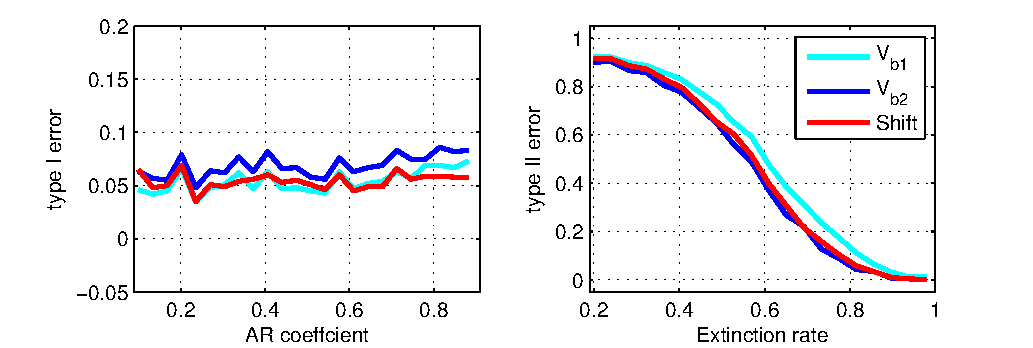
\includegraphics[width=1\textwidth]{arExtinct.pdf}
\caption{Comparison of Shift-HSIC and tests based on $V_{b1}$ and $V_{b2}$. Left panel show the performance under the null hypothesis, larger AR component implies a stronger temporal dependence. Right panel show the performance under the alternative hypothesis, larger extinction rate implies a greater dependence between processes.}
\label{fig:arExtinct}
\end{figure}

\begin{figure}
\centering  
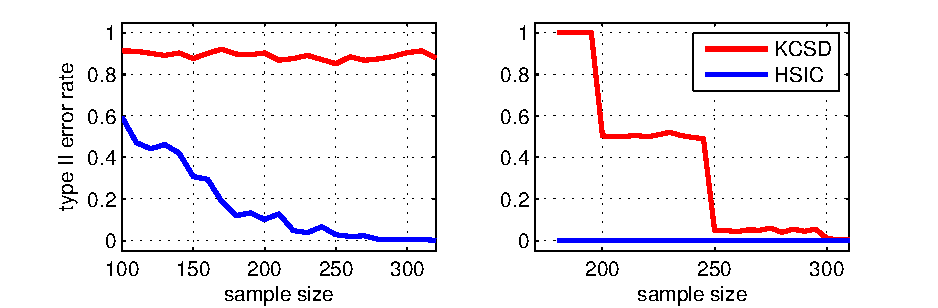
\includegraphics[width=1\textwidth]{varAndPhase.pdf}
\caption{In both panel Type II error is plotted. The left panel presents error of the lag-HSIC and KCSD algorithms for process following dynamics given by the equation \eqref{eq:dynamics2}, whereas the errors for process with dynamics given by equation \eqref{eg:dymamics1a} and \eqref{eg:dymamics1b} are shown in the right panel. X axis is indexed by the time series length i.e. sample size.}
\label{fig:phaseAndVar}
\end{figure}

\vspace{-0.2cm}
\paragraph{The MCMC M.D.}
It is natural to use MMD in order to measure how far the MCMC chain is from its stationary distribution \cite[Section 5]{sejdinovic_KAMH}, 
by comparing the produced sample to a benchmark sample. However, a hypothesis test on whether the sampler has converged based on the standard permutation-based bootstrap leads to too many rejections of the null hypothesis, due to chain dependence. Thus, one would require heavily thinned chains, which is wasteful of samples and computationally burdensome.
Our experiments indicate that the wild bootstrap approach allows consistent tests as it attains a desired number of false positives.\\
To assess performance of the wild bootstrap in MCMC convergence diagnostics, we consider the situation where samples $\{X_i\}$ and $\{Y_i\}$ are bivariate and both have the identical marginal distribution given by an elongated normal
$P=\mathcal{N}\left(\left[\protect\begin{array}{cc}
0 & 0\protect\end{array}\right],\left[\protect\begin{array}{cc}
15.5 & 14.5\protect\\
14.5 & 15.5
\protect\end{array}\right]\right)$.
However, they could have arisen either as independent samples or as outputs of the Gibbs sampler with stationary distribution $P$. 
Table \ref{tab:gibbs_mmd} shows the \emph{rejection rates} under the significance level $\alpha=0.05$. It is clear that in the case where at least one of the samples is a Gibbs chain, the permutation-based test has a Type I error much larger than $\alpha$. 
The wild bootstrap using $V_{b1}$ (without artificial degeneration) yields the correct Type I error control in these cases. Consistent with findings in \cite[Section 5]{leucht_dependent_2013}, $V_{b1}$ mimics the null distribution better than $V_{b2}$. Bootstrapped statistic $\widehat{\text{MMD}}_{k,b}$ in \eqref{eq:mmdkb} which also relies on the artificially degenerated bootstrap processes behaves similarly to $V_{b2}$.
In the alternative scenario where $\{Y_i\}$ was taken from a distribution with the same covariance structure but with the mean set to $\mu= \left[\protect\begin{array}{cc}
2.5 & 0\protect\end{array}\right]$, Type II error for all tests was zero.
\vspace{-0.2cm}
\paragraph{Pitch-evoking sounds}
The second experiment we consider is a two sample test on sounds studied in the field of pitch perception \cite{hehrmannthesis}. We synthesise the sounds with the fundamental frequency
parameter of treble C, subsampled at 10.46kHz. Each $i$-th period
of length $\Omega$ contains $d=20$ audio samples at times $0=t_{1}<\ldots<t_{d}<\Omega$
-- we treat this whole vector as a single observation $X_{i}$ or
$Y_{i}$, i.e., we are comparing distributions on $\mathbb{R}^{20}$.
Sounds are generated based on the AR process $a_{i}=\lambda a_{i-1}+\sqrt{1-\lambda^{2}}\epsilon_{i}$,
where $a_{0},\epsilon_{i}\sim\mathcal{N}(0,I_{d})$, with $X_{i,r}=\sum_{j}\sum_{s=1}^{d}a_{j,s}\exp\left(-\frac{\left(t_{r}-t_{s}-(j-i)\Omega\right)^{2}}{2\sigma^{2}}\right)$,
i.e., a given pattern -- a smoothed version of $a_{0}$ -- slowly
varies and thus the sound deviates from
periodicity, but still evokes a pitch. We take
$X$ with $\sigma=0.1\Omega$
and $\lambda=0.8$, and $Y$ is either an independent copy of $X$
(null scenario), or has $\sigma=0.05\Omega$ (alternative scenario)%
\footnote{Such variation in the smoothness parameter changes the width of the
spectral envelope, i.e., the brightness of the sound.}. $n_x$ is taken to be different from $n_y$. Results in Table \ref{tab:gibbs_mmd} demonstrate how the
approach using the wild bootstrapped statistic in \eqref{eq:mmdkb} allows to control the Type I error and reduce the Type II error with the increasing sample size, while the permutation test
virtually always rejects the null hypothesis.

% \begin{table}
% \caption{Type I error for independent
% samples and Gibbs chains with identical marginal distributions; sample size=500, averaged over 200 trials. Wild bootstrap
% uses blocksize of $l_n=20$. A gaussian kernel with bandwidth
% $\sigma=1.7$ is used. Every second Gibbs sample is kept (i.e., after a pass
% through both dimensions).}
% \label{tab:gibbs_mmd}
% 
% \centering{}%
% \begin{tabular}{|c|c|c|c|c|}
% \hline 
% $X$ vs $Y$ & vanilla & $V_{b1}$ & $V_{b2}$ & $\widehat{\text{MMD}}_{k,b}$\tabularnewline
% \hline 
%  i.i.d. vs i.i.d.  & .040 & \textbf{.012}  & .070 & .025\tabularnewline
% \hline 
% i.i.d. vs Gibbs & .528  & \textbf{.052} & .105 & .100\tabularnewline
% \hline 
% Gibbs vs Gibbs & .680  & \textbf{.060} & .100 & .110\tabularnewline
% \hline 
% \end{tabular}
%\end{table}


\vspace{-0.2cm}
\paragraph{Instantaneous independence}
To examine instantaneous independence test performance we compare it with the Shift-HSIC procedure \cite{chwialkowski2014kernel} on the 'Extinct Gaussian' autoregressive process proposed in the \cite[Section 4.1]{chwialkowski2014kernel}. Using exactly the same setting we compute type I error as a function of the temporal dependence and type II error as a function of extinction rate \footnote{larger extinction rate implies a greater dependence between processes; larger AR component implies a stronger temporal dependence}. The Figure \ref{fig:arExtinct} shows that all three tests, Shift-HSIC and tests based on $V_{b1}$ and $V_{b2}$, perform similarly.   
\vspace{-0.2cm}
\paragraph{Lag-HSIC}
The KCSD  \cite{besserve_statistical_2013} is, to our knowledge, the only procedure to reject the null hypothesis if there exists $t$,$t'$ such that $Z_t$ and $Z_{t'}$ are depended. In the experiments, we compare lag-HSIC with KCSD on two kinds of processes: one  inspired by econometrics and one from \cite{besserve_statistical_2013}.\\ 
In lag-HSIC, the amount of lags under examination was equal to $\max\{10,\log n\}$, where $n$ is the sample size. We have used gaussian kernels with widths estimated by the median heuristic. The cumulative distribution of the $V$-statistics was approximated by samples from $n V_{b2}$. To model the tail of this distribution, we have fitted the generalized Pareto distribution to the bootstrapped samples (\cite{pickands1975statistical} shows that for a large class of underlying distribution functions such an approximation is valid).\\
The first process is a pair of two time series which share a common variance,   
\begin{align}
\label{eq:dynamics2}
 X_t = \epsilon_{1,k} \sigma_k^2, \quad  Y_t = \epsilon_{2,k}  \sigma_k^2,  \quad \sigma_k^2 = 1 + 0.45(X_t^2 + Y_t^2 ).
\end{align}
The above set of equations is an instance of the VEC dynamics \cite{bauwens_multivariate_2006} used in econometrics to model market volatility. The left panel of the Figure \ref{fig:phaseAndVar} presents the Type II error rate: for KCSD it remains at 90\% while for lag-HSIC it gradually drops to zero. The Type I error, which we calculated by sampling two independent copies $(X^{(1)}_{t},Y^{(1)}_{t})$ and $(X^{(2)}_{t},Y^{(2)}_{t})$ of the process and performing the tests on the pair $(X^{(1)}_{t},Y^{(2)}_{t})$, was around 5\% for both of the tests.\\
Our next experiment is a process sampled according to the dynamics proposed by \cite{besserve_statistical_2013},      
\begin{alignat}{2}
  \quad X_k &= \cos(\phi_{k,1})   &\quad  \phi_{k,1} &= \phi_{k-1,1} + 0.1\epsilon_{1,k} + 2 \pi f_1 T_s \label{eg:dymamics1a} \\  
  Y_k &= [2+C\sin(\phi_{k,1})]\cos(\phi_{k,2})  &   \phi_{k,2} &= \phi_{k-1,2} + 0.1\epsilon_{2,k} + 2 \pi f_2 T_s \label{eg:dymamics1b}
\end{alignat}
with parameters $C=.4$, $f_1=4Hz$,$f_2=20Hz$, and frequency $\frac {1} {T_s} = 100 Hz$. We compared performance of the KCSD algorithm, with parameters set to vales recommended in \cite{besserve_statistical_2013}, and the lag-HSIC algorithm. The Type II error of lag-HSIC, presented in the right panel of the Figure \ref{fig:phaseAndVar}, is substantially lower than that of KCSD. The Type I error ($C=0$) is equal or lower than 5\% for both procedures. Most oddly, KCSD error seems to converge to zero in steps. This may be due to the method relying on a spectral decomposition of the signals across a fixed set of bands. As the number of samples increases, the quality of the spectrogram will improve, and dependence will become apparent in bands where it was undetectable at shorter signal lengths.
 


\small
\bibliographystyle{plain}
\bibliography{nips14Bib}

\newpage
\normalsize
\appendix
\section{Proofs}

\subsection{Auxiliary results }
\label{label:aux}
The following section lists all auxiliary Lemmas required to prove main results. We had to extract common parts from the proof of main Theorems in order to make them readable. Therefore we recommend reading Lemma \ref{lem:Components} and the note about notation underneath it first, then main proofs from the sections \ref{sec:prMainOne} and \ref{sec:prMainTwo} and finally this list of Lemmas. 

\begin{proposition}{\cite[p.259, Equation 2.1]{leucht_dependent_2013}}
\label{prop:Coupling}
If process  $\{Z_t,\mathcal{F}_t\}_{t \in \mathbb{N}}$  is $\tau$-dependent and $\mathcal{F}$ is rich enough (see \cite[Lemma 5.3]{dedecker2007weak}), then there exists, for all $t<t_1<...<t_l$, $l \in \mathbb N$, a random vector $(Z_{t_1}^*,...,Z_{t_l}^*)$ that is independent of $\mathcal F_t$, has the same distribution  as $(Z_{t_1},...,Z_{t_l})$ and 
\begin{align*}
\ev \norm{(Z_{t_1}^*,...,Z_{t_l}^*) - (Z_{t_1},...,Z_{t_l})}_1 \leq l \tau(t_1-t).
\end{align*}
\end{proposition}

\begin{lemma}
\label{lem:complicated}
Let $\{Z_i,\mathcal{F}_i\}$ be a $\tau$-mixing sequence,$\{ \delta_i \}$ a sequence of $i.i.d$ random variables independent of filtration $\mathcal{F}$, a non-deceasing sequence $(i_1\leq ... \leq i_m)$, a positive integer $k$ such that $1 < k<m$ and some random vector $(Z_{i_1},...,Z_{i_m})$. Further let $A = (Z_{i_1},...,Z_{i_{k-1}})$, $B= Z_{i_k}$ and $C=(Z_{i_{k+1}},...,Z_{i_{m}})$,  $\mathcal{F_A} =\mathcal{F}_{k-1}$, $\mathcal{F_B}  =\mathcal{F}_{k}$. There exist independent random variables $B^*$ and $C^*$, independent of $\mathcal{F_A}$, such that  
\begin{align}
\ev |B-B^*| = \tau(i_{k} -i_{k+1}) \text{ and } \frac{1} {m-k} \ev \parallel C-C^* \parallel_1 \leq \tau(i_{k+1}-i_k) 
\end{align}    
\end{lemma}


\begin{proof}
We first use use  \cite[Equation 2.1]{leucht_dependent_2013}] (also \cite[Lemma 5.3]{dedecker2007weak}) to construct $C^*$ such that $\frac{1} {m-k}  \ev \parallel C-C^* \parallel_1 \leq (m-k) \tau(i_{k+1}-i_k)$. By construction $C^*$ is independent of $\mathcal{F_B}$. Since $ \mathcal{F_A} \subset \mathcal{F_B}$ and $ \sigma(B) \subset \mathcal{F_B}$ and $C^* \indep (\sigma(\delta_k) $, then $C^* \indep  (\mathcal{F_A} \vee \sigma(B)  \vee \sigma(\delta_k)  )$. Next by \cite[Lemma 5.2]{dedecker2007weak} we construct $B^*$  such  that $\ev |B-B^*| = \tau(i_{k} -i_{k+1})$, and $B^*$  independent  of $\mathcal{F_A}$ but $\mathcal{F_A} \vee \sigma(B) \vee \sigma(\delta_k)$ measurable. Since   $\sigma(C^*) \indep (\mathcal{F_A} \vee \sigma(B) \vee \sigma(\delta)) $ then $C^*$ and $B^*$ are independent. Finally both $C^*$ and $B^*$ are independent of $\mathcal{F_A}$   
\end{proof}

\begin{lemma}
\label{lem:Components}\cite[Section 5.1.5]{serfling80}
Any core $h$ can be written as a sum of canonical cores $h_1,...,h_m$ and a constant $h_0$
\begin{align*}
h(z_1,...,z_m) &=   h_m(z_1,...,z_m) + \sum_{1 \leq i_1 < ...<i_{m-1} \leq m } h_{m-1}(z_{i_1},...,z_{i_{m-1}}) \\ 
    & + ... + \sum_{1 \leq i_1 < i_2 \leq m } h_2(z_{i_1},z_{i_2}) + \sum_{1 \leq i \leq m} h_1(z_i)+h_0
\end{align*} 
\end{lemma}

\begin{proof}
To show this we define auxiliary functions
\[
 g_c(z_1,...z_c) = \ev h(z_1,...,z_c,Z_{c+1}^*,...,Z_{m}^*)
\]
for each $c=0,...,m-1$ and put $g_m=h$.  

Canonical functions that allow core decomposition are 
\begin{align}
   h_0 &= g_0, \\  
   h_1(z_1) &= g_1(z_1) -h_0,\\
   h_2(z_1,z_2) &= g_2(z_1,z_2)  - h_1(z_1) - h_1(z_2)-h_0, \\  
   h_3(z_1,z_2,z_3) &= g_3(z_1,z_2,z_3) - \sum_{1 \leq i < j \leq 3 } h_2(z_i,z_j) - \sum_{1\leq i \leq 3} h_1(z_i)-h_0, \\ 
   \cdots &, \\
   h_m(z_1,...,z_m) &= g_m(z_1,...,z_m) - \sum_{1 \leq i_1 < ...<i_{m-1} \leq m } h_{m-1}(z_{i_1},...,z_{i_{m-1}}) \\ 
    & - ... - \sum_{1 \leq i_1 < i_2 \leq m } h_2(z_{i_1},z_{i_2}) - \sum_{1 \leq i \leq m} h_1(z_i)-h_0.\\
\end{align}
Lemma \ref{lem:symetric} shows that functions $h_c$ are symmetric (and therefore cores) and Lemma \ref{stm:coreDegeneracy} shows that they are canonical.  
\end{proof}

\textbf{ We call $h_1,...,h_m$ components of a core $h$. We do not call $h_0$ a component, its simply a constant.}
 
 
 
 
\begin{lemma}\cite[Section 5.1.5]{serfling80}
\label{lem:symetric}
Components of a core $h$ are symmetric functions.
\end{lemma}
%\begin{proof}
%We will use induction by components' index to show that $h_c$ is symmetric. $h_1$ is a function of one argument, hence it is symmetric. Suppose that for each $c' < c$ component $h_{c'}$ is symmetric. Each sum 
% \begin{align}
%  \sum_{1 \leq i_1 < ...<i_{c} \leq c } h_{c'}(z_{i_1},...,z_{i_{c'}}) 
% \end{align}
%is symmetric with respect to arguments $z_1,...,z_c$. $g_c(z_1,...,z_c)$ symmetry follows from $h$ symmetry. Hence function 
%\begin{align}
%   h_c(z_1,...,z_c) &= g_c(z_1,...,z_c) - \sum_{1 \leq i_1 < ...<i_{c-1} \leq c } h_{c-1}(z_{i_1},...,z_{i_{c-1}}) \\ 
%    & - ... - \sum_{1 \leq i_1 < i_2 \leq c } h_2(z_{i_1},z_{i_2}) - \sum_{1 \leq i \leq c} h_1(z_i) - h_0.\\
%\end{align}
%is symmetric as a sum of expressions symmetric with respect to  arguments $z_1,...,z_c$. 
%\end{proof}






\begin{lemma}\cite[Section 5.1.5]{serfling80}
\label{stm:coreDegeneracy}
 A component of a core $h$ is a canonical core. 
\end{lemma}
%\begin{proof}
% We will use induction by components' index to show that $h_c$ is canonical. Expected value of the first component is zero, indeed $\ev h_1(Z_1^*)= \ev h(Z_1^*,...,Z_m^*)  -h_0= 0$. Suppose that for all $c'$ smaller then $c$ degeneracy holds. If  $\ev h_c(z_1,...,z_{c-1},Z_c^*)=0$ then for any $k$, $\ev h_c(z_1,...,Z_k^*,...,z_{c})=0$ since $h_c$ is symmetric, hence it is enough to show that $\ev h_c(z_1,...,z_{c-1},Z_c^*)=0$. Consider a sum
%\begin{align}
%  &\sum_{1 \leq i_1 < ...<i_{c'} \leq c }   h_{c'}(z_{i_1},...,z_{i_{c'}}) = \\
%  \sum_{1 \leq i_1 < ...<i_{c'} \leq c-1 }  &h_{c'}(z_{i_1},...,z_{i_{c'}}) +  \sum_{1 \leq i_1 < ...<i_{c'-1} < c }  h_{c'}(z_{i_1},...,z_{c}).
%\end{align}
%The left hand side sum $\sum_{1 \leq i_1 < ...<i_{c'} \leq c-1 } h_{c'}(z_{i_1},...,z_{i_{c'}})$ does not contain term $z_c$ so integration with respect to $Z_c^*$ does not affect it. On the other hand, by the inductive assumption $\ev \sum_{1 \leq i_1 < ...<i_{c'-1} < c }  h_{c'}(z_{i_1},...,Z_{c}^*) = 0$ and by $g_c$ definition $\ev g_c(z_1,...,Z_{c}^*) =  g_{c-1}(z_1,...,z_{c-1})$. Using these observations we simplify 
%\begin{align}
%  \ev h_c(z_1,...,Z_{c}^*) &=  g_{c-1}(z_1,...,z_{c-1}) -  \sum_{1 \leq i_1 < ...<i_{c-1} \leq c-1 } h_{c-1}(z_{i_1},...,z_{i_{c-1}}) \\
%   & - ... -  \sum_{1 \leq i_1 < i_2 \leq c-1 }   h_2(z_{i_1},z_{i_2}) -  \sum_{i=1}^{c-1}  h_1(z_i)  - h_0.\\
%\end{align}
%Since the  set  $ \{1 \leq i_1 < ...<i_{c-1} \leq c-1 \}$ contains only one sequence we can write  
%\begin{align}
%   \ev h_c(z_1,...,Z_{c}^*) &= -  h_{c-1}(z_{i_1},...,z_{i_{c-1}}) + \big[ g_{c-1}(z_1,...,z_{c-1})  \\
%   & - ... -  \sum_{1 \leq i_1 < i_2 \leq c-1 }   h_2(z_{i_1},z_{i_2}) -  \sum_{i=1}^{c-1}  h_1(z_i) - h_0\big] =0.\\
%\end{align}
%For this nice simplification we have used the definition of the component $h_{c-1}$.
%\end{proof}






\begin{lemma}
\label{stm:LipAndBound}
 If $h$ is bounded and Lipschitz continuous core then its components are also bounded and Lipschitz continuous.
\end{lemma}
\begin{proof}
 Note that 
\begin{align}
g_c(z_1,...z_c) = \ev h(z_1,...,z_c,Z_{c+1}^*,...,Z_{m}^*) \leq \ev \parallel h \parallel_{\infty}.  
\end{align}
To prove boundedness  we use induction - we assume that components with low index are bounded and use the fact that sum of bounded functions is bounded to obtain the required results.
We prove Lipschitz continuity similarly, first by showing that $g_c(z_1,...z_c)$ are Lipschitz continuous with the same coefficient as the core $h$ and then by using the fact that sum of Lipschitz continuous functions  is  Lipschitz continuous.
\end{proof}


\begin{lemma}
\label{lem:summingLema}
If $1 \leq  j_k,r_j \leq m$ are disjoint sequences with respectively $q$ and $m-q$ elements, such that elements in each sequence are unique then
\begin{align}
\sum_{i \in N^m} f(Z_{i_{j_1}},...,Z_{i_{j_q}}) = n^{m-q} \sum_{i \in N^q} f(Z_{i_1},...,Z_{i_q})
\end{align}
\end{lemma}
\begin{proof}
\begin{align}
&\sum_{i \in N^m} f(Z_{i_{j_1}},...,Z_{i_{j_q}}) = \sum_{1 \leq i_{j_1},...,i_{j_q} \leq n}  \sum_{1 \leq i_{r_1},...,i_{r_{m-q}} \leq n} f(Z_{i_{j_1}},...,Z_{i_{j_q}}) = \\
&\sum_{1 \leq i_{j_1},...,i_{j_q} \leq n}  \left( f(Z_{i_{j_1}},...,Z_{i_{j_q}})  \sum_{1 \leq i_{r_1},...,i_{r_{m-q}} \leq n} 1 \right) =\\
&n^{m-q} \sum_{1 \leq i_{j_1},...,i_{j_q} \leq n}   f(Z_{i_{j_1}},...,Z_{i_{j_q}})  =n^{m-q} \sum_{i \in N^q} f(Z_{i_1},...,Z_{i_q}).
\end{align}
\end{proof}




\begin{lemma}
\label{stm:decomposition}[Section 5.1.5]
 V-statistic of a core function h can be written as a sum of  V-statistics with canonical cores
\begin{align}
  V(h) = V(h_m) + \binom m 1 V(h_{m-1}) + ...+ \binom {m} {m-2} V(h_{2}) + \binom {m} {m-1} V(h_{1}) + h_0.
 \end{align}
\end{lemma}
%\begin{proof}
%\begin{align}
%V(h)& = \frac{1} {n^m} \sum_{i \in N^m} h(Z_{i_1},...,Z_{i_m}) = \\
%& \frac{1} {n^m}  \sum_{i \in N^m}   \left( h_m(Z_1,...,Z_m) + \sum_{1 \leq j_1 < ...<j_{m-1} \leq m } h_{m-1}(Z_{i_{j_1}},...,Z_{i_{j_{m-1}}}) \right. \\ 
%    & \left. + ... + \sum_{1 \leq j_1 < j_2 \leq m } h_2(Z_{i_{j_1}},Z_{i_{j_2}}) + \sum_{1 \leq j \leq m} h_1(Z_{i_j}) + h_0\right) \overset{L.\ref{lem:summingLema}}{=\joinrel=} \\
%    & \frac{1} {n^m}  \sum_{i \in N^m}   h_m(Z_1,...,Z_m) +  \binom m 1 \frac{1} {n^{m-1}}  \sum_{i \in N^{m-1}} h_{m-1}(Z_{i_1},...,Z_{i_{m-1}}) + \\
%    & + ... + \binom {m} {m-2} \frac{1} {n^2}  \sum_{i \in N^2} h_2(Z_{i_1},Z_{i_2}) +  \binom {m} {m-1} \frac{1} {n} \sum_{i \in N} h_1(Z_i) + h_0= \\
%    &V(h_m) + \binom m 1 V(h_{m-1}) + ...+ \binom {m} {m-2} V(h_{2}) + \binom {m} {m-1} V(h_{1}) + h_0.
%\end{align}
%\end{proof}


\begin{lemma}
\label{lem:start}
Assume that the stationary process $Z_t$ is $\tau$-dependent with a coefficient $\tau(i) = i^{-6-\epsilon}$ for some $\epsilon>0$. If $h$ is a canonical and Lipschitz continuous core of three arguments then
 \begin{align}
 \lim_{n \to \infty} \frac{1}{n^2} \sum_{i \in N^{m}} |\ev   h(Z_{i_1},Z_{i_2},Z_{i_3})| =0.
\end{align}
converges to zero in probability.
\end{lemma}

\begin{proof}
We change summing order, it is useful to think of index $b$ as 'beginning', $e$ as 'end' and $m$ as 'middle'. 
 \begin{align}
 \label{eq:143}
 \sum_{i \in N^{m}} |\ev   h(Z_{i_1},Z_{i_2},Z_{i_3})| =  3! \sum_{b=1}^n \sum_{e=b}^n \sum_{b \leq m \leq e }^n |\ev   h(Z_b,Z_m,Z_e)|.
\end{align}
For each $b,m,e$, $|\ev   h(Z_b,Z_m,Z_e)| \leq 2 \tau(max(e-m,m-b))$. To see that suppose that $m-b>e-m$. Then by Proposition \ref{prop:Coupling} there exists random vector $(Z_m^*,Z_e^*)$ independent of $Z_b$ such that $\frac 1 2 \ev \parallel (Z_m^*,Z_e^*) - (Z_m,Z_e) \parallel \leq \tau(m-b)$. Furthermore 
\begin{align}
 |\ev   \left(   h(Z_b,Z_m,Z_e) -  h(Z_b,Z_m^*,Z_e^*) + h(Z_b,Z_m^*,Z_e^*) \right) | \leq  \\
 |\ev   \left(   h(Z_b,Z_m,Z_e) -  h(Z_b,Z_m^*,Z_e^*) \right) |+ |\ev h(Z_b,Z_m^*,Z_e^*) | \leq Lip(h) 2\tau(m-b) +0, 
\end{align}
since $\ev h(Z_b,Z_m^*,Z_e^*)=0$. Similar reasoning for case $m-b<e-m$ proofs that $|\ev h(Z_b,Z_m,Z_e)| \leq 2 Lip(h) \tau(max(e-m,m-b))$. Since $max(e-m,m-b)>(e-b)/2$   
\begin{align}
3! \sum_{b=1}^n \sum_{e=b}^n \sum_{b \leq m \leq e }^n |\ev h(Z_b,Z_m,Z_e)| \leq 12 Lip(h) \sum_{b=1}^n \sum_{e=b}^n \sum_{b \leq m \leq e }^n \tau((e-b)/2) \leq  \\ 
12 Lip(h) \sum_{b=1}^n \sum_{e=b}^n (e-b) \frac{8} {(e-b)^3} \leq 96 Lip(h) \sum_{b=1}^n \sum_{e=b}^n \frac{1} {(e-b)^2} = O(n).
\end{align}
\end{proof}


\begin{lemma}
\label{lem:missingBit}
Assume that the stationary process $Z_t$ is $\tau$-dependent with a coefficient $\tau(i) = i^{-6-\epsilon}$ for some $\epsilon>0$. If $h$ is Lipschitz continuous function of $m$ arguments, $m>3$, such that for any $1 \leq k \leq m$
\begin{align}
\label{eq:assumptionCanonical}
\ev h(z_1,...,Z_k,...,z_m) =0
\end{align}
then
\begin{align}
 \lim_{n \to \infty} \frac{1}{n^{m-2}} \sum_{i \in N^{m}} |\ev   h(Z_{i_1},...,Z_{i_m})| =0.
\end{align}
converges to zero in probability.
\end{lemma}

\begin{proof}
 The proof follows proof by \cite[Lemma 3]{arcones1998law}. 
\begin{align}
 \sum_{i \in N^{m}} |\ev   h(Z_{i_1},...,Z_{i_m})| \leq \sum_{\pi \in S_m} \sum_{1 \leq i_1< ...\leq i_m \leq n} |\ev   h(Z_{i_{\pi(1)}},...,Z_{i_{\pi(m)}})|
\end{align}
where $S_m$ is group of permutations of $m$ elements.  Let, $g=\lfloor m/2 \rfloor$ , $j_1 = i_2 - i_1$ , let $j_l = min(i_{2l-1} - i_{2l-2} , i_{2l} - i_{2l-1} )$ for $2 \leq l \leq g$  and let $j_g = i_m - i_{m-1}$ if $m$ is even. If $j_1$ is equal to $max(j_1,...,j_g)$ then we use Proposition \ref{prop:Coupling} and, by the reasoning similar to one in the  Lemma \ref{lem:start} ), we obtain bound
 \begin{align}
  |\ev   h(Z_{i_{\pi(1)}},...,Z_{i_{\pi(m)}})| \leq \tau(j_1). 
 \end{align}
Same reasoning holds if $j_g$ is equal to $max(j_1,...,j_g)$ and $m$ is even. In other case there exists $1 < k \leq g$ for which maximum is obtained. Let
\begin{align}
A &= (Z_{i_1},...,Z_{i_{2k-1}}) \\
B &= Z_{i_{2k}} \\
C &= (Z_{i_{2k+1}},...,Z_{i_m}) )\\
h(A,B,C) &= h(Z_{i_{\pi(1)}},...,Z_{i_{\pi(2k-1)}},Z_{i_{\pi(2k)}},Z_{i_{\pi(2k+1)}},...,Z_{i_\pi(m)}).
\end{align}
And $B^*$,$C$ are as in Lemma \ref{lem:complicated}. We use Lemma \ref{lem:complicated} to see that 
\begin{align}
&  |\ev   h(A,B,C)| \leq | \ev ( h(A,B,C) -  h(A,B^*,C^*)| +  |\ev h(A,B^*,C^*)| = \\
&= | \ev ( h(A,B,C) -  h(A,B^*,C^*)| + 0  \leq Lip(h)  \tau(j_k).
\end{align}
For second equality we have used assumption \ref{eq:assumptionCanonical} and that $B^*$ is independent of $A$ and $C^*$. Therefore we showed that if $w=max(j_1,...,j_g)$
\begin{align}
| \ev h(Z_{i_{\pi(1)}},...,Z_{i_{\pi(m)}}) | \leq \tau(w).
\end{align}

Now for each $w=1$ to $n$ we count all possible combinations of indexes $i_1$ to $i_m$. Suppose $w=max(j_1,...,j_g)$ and that it is obtained at first position i.e. $j_1=w$. Then $i_1$ can take at most $n$ positions and position of $i_2$ is fixed. If $i_3-i_2 \leq i_4- i_3$ then $i_3 \leq w +i_2$ and therefore $i_3$ can take at most $w$ values and $i_4$ can take at most $n$ values. On the other hand if  $i_3-i_2 \geq i_4- i_3$ then $i_4$ can take at most $w$ values and $i_3$ can take at most $n$ values. Proceeding in this way we obtain that the possible values for the variables $i_1 \leq ... \leq i_m$. In case $m$ is even number of combinations of $i_1,...,i_m$ is smaller than $n^{g}w^{g-1}$ and in case $m$ is odd number of combinations is smaller than $n^g w^{g}$. 

If $j_k=max(j_1,...,j_g)$ for $1 < k \leq g$ similar reasoning holds - we bound number of combinations for the first triple $(i_1,i_2,i_3)$, second triple $(i_3,i_4,i_5)$ etc. 

There are $O(n)$ combinations for $w=0$ and since $\parallel h \parallel_{\infty} \leq \infty$ sum over them is of order $n$. Therefore for values of $w$ varying in a range $1$ to $n-1$ we have 
\begin{align}
 \sum_{\pi \in S_m} \sum_{1 \leq i_1< ...\leq i_m \leq n} |\ev   h(Z_{i_{\pi(1)}},...,Z_{i_{\pi(m)}})|  \leq \\
n^g \left( \sum_{w=1}^{n-1} w^g \tau(g) \right) + O(n)  \leq  n^g \left( \sum_{w=1}^{n-1} w^{g-4} \right)+O(n) = O( n^{2g-3}) = O( n^{m-3}).
\end{align}
\end{proof}


\begin{corollary}
\label{lem:auxAsymp1}
Assume that the stationary process $Z_t$ is $\tau$-dependent with a coefficient $\tau(i) = i^{-6-\epsilon}$ for some $\epsilon>0$. If $h$ is a canonical and Lipschitz continuous core of three or more arguments, then 
\begin{align}
 \lim_{n \to \infty} \frac{1}{n^{m-1}} \sum_{i \in N^{m}} |\ev   h(Z_{i_1},...,Z_{i_m})| =0.
\end{align}
\end{corollary}




\begin{lemma}
\label{lem:auxAsymp2}
Assume that the stationary process $Z_t$ is $\tau$-dependent with a coefficient $\tau(i) = i^{-6-\epsilon}$ for some $\epsilon>0$. If $h$ is a canonical and Lipschitz continuous core of three or more arguments, then
\[
  \lim_{n \to \infty}\frac{1} {n^{2m-2}}   \sum_{i \in N^{2m}} \ev |h(Z_{i_1},...,Z_{i_m})h(Z_{i_{m+1}},...,Z_{i_{2m}})| = 0.
\]
\end{lemma}
\begin{proof}
Let $g(z_{i_1},...,z_{i_m},z_{i_{m+1}},...,z_{i_{2m}})=h(z_{i_1},...,z_{i_m})h(z_{i_{m+1}},...,z_{i_{2m}})$. Since $h$ is canonical $g$ meets assumptions of the Lemma \ref{lem:missingBit} from which the Proposition follows.
\end{proof}





\begin{lemma}
\label{lem:auxAsymp2a}
Assume that the stationary process $Z_t$ is $\tau$-dependent with a coefficient $\tau(i) = i^{-6-\epsilon}$ for some $\epsilon>0$. Let $h$ be a canonical and Lipschitz continuous core of $c$ arguments, $3 \leq c \leq m$, and $1 \leq j_1 < ...<j_c \leq m$ be a sequence of $c$ integers. If $Q_{i_1,...,i_m}$ is a random variable independent of $(Z_{i_1},...,Z_{i_m})$ such that $\sup_{i \in N^m} \ev |Q_i| \leq \infty$ and $\sup_{i \in N^{m}} \sup_{o \in N^m} \ev |Q_i Q_o| \leq \infty$  then 
\begin{align}
&\lim_{n \to \infty}\frac{1} {n^{m-1}} \ev  \sum_{i \in N^{m}}  Q_i h(Z_{i_{j_1}},...,Z_{i_{j_c}}) \overset{P}{=} 0. \\
&\lim_{n \to \infty}\frac{1} {n^{2m-2}} \ev  \sum_{i \in N^{m}} \sum_{o \in N^{m}}  Q_i Q_o h(Z_{i_{j_1}},...,Z_{i_{j_c}}) h(Z_{i_{o_1}},...,Z_{i_{o_c}}) \overset{P}{=} 0. \\
\end{align}
For the first limit notice  that 
\begin{align}
&\frac{1} {n^{m-1}} \ev  \sum_{i \in N^{m}}  Q_i h(Z_{i_{j_1}},...,Z_{i_{j_c}}) \leq  \frac{1} {n^{m-1}}  \sum_{i \in N^{m}}  |\ev Q_i| |\ev h(Z_{i_{j_1}},...,Z_{i_{j_c}})| \overset{ \ref{lem:summingLema}}{\leq} \\
& \sup_{i \in N^m} |\ev Q_i|   \frac{1} {n^{c-1}}  \sum_{i \in N^c} |\ev h(Z_{i_1},...,Z_{i_c})| \overset{\ref{lem:auxAsymp1}}{\longrightarrow} 0 \text{  in probablity}. 
\end{align}
Similar reasoning, which uses Lemma \ref{lem:auxAsymp2} instead of \ref{lem:auxAsymp1}, shows convergence of the second limit. 
\end{lemma}


\begin{lemma}
\label{lem:higherVstats}
Assume that the stationary process $Z_t$ is $\tau$-dependent with a coefficient $\tau(i) = i^{-6-\epsilon}$ for some $\epsilon>0$. Let $h$ be a canonical and Lipschitz continuous core of $c$ arguments, $3 \leq c \leq m$. If $Q_{i_1,...,i_m}$ is a random variable independent of $(Z_{i_1},...,Z_{i_m})$ such that $\sup_{i \in N^m} \ev |Q_i| \leq \infty$ and $\sup_{i \in N^{m}} \sup_{o \in N^m} \ev |Q_i Q_o| \leq \infty$  then 
\begin{align}
\lim_{n \to \infty} \frac {1} {n^{m-1}} \sum_{i \in N^m}  \sum_{1 \leq j_1<...<j_c < m} \ev Q_i   h_c(Z_{i_{j_1}},...,Z_{i_{j_c}}) \overset{P}{=} 0.
\end{align}
\end{lemma}
\begin{proof}
For each sequence such that  $1 \leq j_1<...<j_c < m$  we apply Lemma \ref{lem:auxAsymp2a} and  conclude that the random sum 
\begin{align}
\frac {1} {n^{m-1}} \sum_{i \in N^m} \ev Q_{i_{j_1},...,i_{j_c}}   h_c(Z_{i_{j_1}},...,Z_{i_{j_c}})
\end{align}
converges to zero in a probability - from this the proposition follows.
\end{proof}


\begin{lemma}
\label{lem:higherVstats2}
Assume that the stationary process $Z_t$ is $\tau$-dependent with a coefficient $\tau(i) = i^{-6-\epsilon}$ for some $\epsilon>0$. If $h$ if a canonical and Lipschitz continuous core of three or more arguments  
\begin{align}
\lim_{n \to \infty} n V(h_c) = 0.
\end{align}
\end{lemma}
\begin{proof}
For each $c$ put $Q=1$ and use Lemma \ref{lem:higherVstats}.
\end{proof}





\begin{lemma}
\label{lem:meanWi}
If $W_i$ is a bootstrap process defined in the section \ref{sec:background} then
\begin{align}
\lim_{n \to \infty} \frac 1 n \sum_{i=1}^n W_i \overset{P}{=} 0.
\end{align}
\end{lemma}
\begin{proof}
By the definition of $W_i$, $\ev (\sum_{i=1}^n W_i)^2 = O(n l_n)$,  $\lim_{n \to \infty} \frac {l_n}{n} =0 $ and $\ev \sum_{i=1}^n W_i = 0$. Therefore $\frac{1} {n} \sum_{i=1}^{n}W_i$ converges to zero in probability.
\end{proof}





\begin{lemma}
\label{lem:toZeroWi}
Assume that the stationary process $Z_t$ is $\tau$-dependent with a coefficient $\tau(i) = i^{-6-\epsilon}$ for some $\epsilon>0$ and $W_i$ is a bootstrap process defined in the section \ref{sec:background}. Let $f$ be a one-degenerate, Lipschitz continuous, bounded core of at least $m$ arguments, $m \geq 2$. Further assume that $f_2$ is a kernel. Then for a positive integer $p$
\begin{align}
\lim_{n \to \infty } n V(f) \left( \frac 1 n \sum_{i=1}^n W_i \right)^p \overset{P}{=} 0
\end{align}
\end{lemma}

\begin{proof}
By  the Lemma \ref{lem:meanWi} $\frac{1} {n} \sum_{i=1}^{n}W_i$ converges to zero in probability. By Theorem \ref{th:mainOne} $ \frac {1}{n^{m-1}} \sum_{i \in N^m} f(Z_{i_m},...,Z_{i_m}) $ converges to some random variable. 
\end{proof}

\begin{lemma}
\label{lem:oneWtrick}
Assume that the stationary process $Z_t$ is $\tau$-dependent with a coefficient $\tau(i) = i^{-6-\epsilon}$ for some $\epsilon>0$ and $W_i$ is a bootstrap process defined in the section \ref{sec:background}. If $h$ is a Lipschitz continuous, degenerate and bounded core of two arguments then 
\begin{align}
\frac{1}{n} \sum_{i \in N^2} W_{i_1} h(Z_{i_1},Z_{i_2}) 
\end{align}
converges in distribution to some random variable.
\end{lemma}
\begin{proof}
\begin{align}
\label{eq:h2eq1}
& \frac{1}{n} \sum_{i \in N^2} W_{i_1}  h(Z_{i_1},Z_{i_3}) = \frac 1 4 (V_{-} + V_{+}) \text{ where,} \\   
V_{-} &= n^{-1} \sum_{i \in N^2} (W_{i_1}-1)h(Z_{i_1},Z_{i_2})(W_{i_2}-1), \\
V_{+} &= n^{-1} \sum_{i \in N^2}  (W_{i_1}+1)h(Z_{i_1},Z_{i_2})(W_{i_2}+1), \\ 
\end{align}
are normalized V statistics that converge. To see that we use Lemma \ref{lem:convergence2012} with $g_{+}(x)=x+1$ and $g_{-}(x)=x-1$ respectively. The only non-trivial assumption is that $\ev|g_{+}(W_i)|^k < \infty$ and $\ev|g_{-}(W_i)|^k<\infty$  - this follows from $\ev |W_i|^k$. 
\end{proof}




\begin{lemma}
\label{lem:convergence2012}
Assume that the stationary process $Z_t$ is $\tau$-dependent with a coefficient $\tau(i) = i^{-6-\epsilon}$ for some $\epsilon>0$ and $W_i$ is a bootstrap process defined in the section \ref{sec:background}. Let $x=(w,z)$ and suppose $f(x_1,x_2) = g(w_1)g(w_2) h(z_1,z_2)$ where $g$ is Lipschitz continuous, $\ev |g(W_1)|^3 \leq \infty$ and $h$ is symmetric, Lipschitz continuous, degenerate and bounded. Then 
\begin{align}
n V(f)= \frac 1 n \sum_{i,j} f(X_i,X_j) = \frac 1 n \sum_{i,j} g(W_i) g(W_j) h(Z_i,Z_j) 
\end{align}
converges to some random variable in law.   
\end{lemma}
\begin{proof}
We use  \cite[Theorem 2.1]{leucht2012degenerate} to show that $n V(f)$ converges that requires checking assumptions $\textit{A1 - A3}$ 

\textit{Assumption A1.} Point (i) requires that the process $(W_n,Z_n)$ is a strictly stationary sequence of $\mathbb{R}^d$-values integrable random variables - this follows from the assumptions. For the point (ii) we put $\delta=\frac 1 3$ and check
\begin{align}
\sum_{r=1}^{\infty} r \tau(r)^{\delta} \leq \sum_{r=1}^{\infty} r r^{-6 \frac 1 3} = \sum_{r=1}^{\infty} r^{-2} < \infty. 
\end{align}

\textit{Assumption A2.} Point (i) requires that the function $f$ is symmetric, measurable and
degenerate. Symmetry and measurability are obvious and for the degeneracy we calculate 
\begin{align}
\ev g(W_1) g(w) h(Z_1,z) =  \ev g(W_1) g(w) \ev h(Z_1,z) = 0.
\end{align}  

 Point (ii) requires that for $\nu > (2-\delta)/(1-\delta) = 2.5$ (since we have chosen $\delta=\frac 1 3$).
\begin{align}
\sup_{k \in \mathbf{N}} \ev |f(X_1,X_k)|^{\nu} < \infty \text{ and } \sup_{k \in \mathbf{N}} \ev |f(X_1,X_k^*)|^{\nu} < \infty
\end{align}
Both requirements are met since $h$ is bounded and the process $\ev |g(W_i)|^3 \leq \infty$ .

\textit{Assumption A3.} Function $f$ is Lipschitz continuous - this is met since both $g$ and $h$ are Lipschitz continuous.   
\end{proof}




\begin{lemma}
\label{stmt:obviousD}
If $W_i$ is a bootstrap process defined in the section \ref{sec:background} then
\begin{align}
\sum_{i=1}^n \tilde W_i = \sum_{i=1}^n  \left( W_i - \frac 1 n \sum_{i=j}  W_j \right) = 0. 
\end{align}
\end{lemma}

\begin{lemma}
\label{lem:convergenceProblem}
Assume that the stationary process $Z_t$ is $\tau$-dependent with a coefficient $\tau(i) = i^{-6-\epsilon}$ for some $\epsilon>0$ and $W_i$ is a bootstrap process defined in the section \ref{sec:background}. If $f$ is canonical, Lipschitz continuous, bounded core then a random variable 
\begin{align}
\frac 1 n  \sum_{1 \leq i,j \leq n} \tilde W_i \tilde W_j f(Z_i,Z_j)
\end{align}
converges in law.
\end{lemma}

\begin{proof}
\begin{align}
&\frac 1 n \sum_{1 \leq i,j \leq n} \tilde W_i \tilde W_j f(Z_i,Z_j) = \frac 1 n \sum_{1 \leq i,j \leq n} \left( W_i - \sum_{a=1}^n W_a \right) \left( W_i - \sum_{b=1}^n W_b \right) f(Z_i,Z_j) =\\
&\frac 1 n \sum_{1 \leq i,j \leq n} W_i W_j f(Z_i,Z_j)  - \left( \frac 2 n \sum_{1 \leq i,j \leq n} f(Z_i,Z_j) \right) \left( \frac 1 n \sum_{b=1}^n W_b \right)  + \left( \frac 1 n  \sum_{1 \leq i,j \leq n} f(Z_i,Z_j) \right) \left( \frac 1 n \sum_{b=1}^n W_b \right)^2.
\end{align}
Last two terms converge to zero since by Lemma \ref{stmt:obviousD} $\left( \frac 1 n \sum_{b=1}^n W_b \right)$ converges to zero and  by the Lemma \ref{lem:convergence2012} (with $g=1$ ) $\frac 1 n  \sum_{1 \leq i,j \leq n} f(Z_i,Z_j)$ converges in law. The first term converges by the Lemma \ref{lem:convergence2012}. 
\end{proof}


%%%%%%%%%%%%%%%%%%%%%%% Proof of the Theorem  \ref{th:mainOne} %%%%%%%%%%%%%%%%%%%%%%%%%%%%%%%
\subsection{Proof of the Theorem  \ref{th:mainOne}} 
 \label{sec:prMainOne}
 
\begin{lemma}
\label{lem:equivVanila}
Assume that the stationary process $Z_t$ is $\tau$-dependent with a coefficient $\tau(i) = i^{-6-\epsilon}$ for some $\epsilon>0$. If core $h$ is Lipschitz continuous, one-degenerate, bounded, and its $h_2$ component is a kernel then its normalized $V$ statistic limiting distribution is proportional to its second component normalized $V$-statistic distribution. Shortly    
\begin{align}
\lim_{n \to \infty} \varphi( n V(h), \binom m 2  n V(h_2) ) = 0. 
\end{align}
where $\varphi$ denotes Prokhorov metric. 
\end{lemma}
\begin{proof}
Lemma \ref{stm:decomposition} shows how to write core  $h$ as a sum of its components $h_i$ ,
\begin{align}
  n V(h) = n V(h_m) + \binom m 1 n V(h_{m-1}) + ...+ \binom {m} {m-2} n V(h_{2}) + \binom {m} {m-1} n V(h_{1})+h_0.
\end{align}
By Lemma \ref{stm:LipAndBound} all components of $h$ are bounded and Lipschitz continuous. Since $h$ is one-degenerate, $h_0=0$ and component $h_1(z)$ is equal to zero everywhere
\begin{align}
h_1(z) = \ev h(z,Z_{2}^*,...,Z_{m}^*)=0. 
\end{align}

By Lemma \ref{lem:higherVstats2}, for $c \geq 3$, $n V(h_{c})$  converges to zero in probability. Therefore the behaviour of $V(h)$ is determined by $\binom {m} {m-2} V(h_2) = \binom {m} {2} V(h_2)$. Convergence of $V(h_2)$ follows from the \cite[Theorem 2.1]{leucht_dependent_2013}.
\end{proof}




\begin{lemma}
\label{lem:equivBoot}
Assume that the stationary process $Z_t$ is $\tau$-dependent with a coefficient $\tau(i) = i^{-6-\epsilon}$ for some $\epsilon>0$. If core $h$ is Lipschitz continuous, one-degenerate, bounded, and its $h_2$ component is a kernel then its normalized and bootstrapped $V$ statistic limiting distribution is same its second component normalized and bootstrapped $V$-statistic distribution. Shortly
\begin{align}
\lim_{n \to \infty} \varphi( n V_b(h), V_b(h_2)) =0. 
\end{align}
where $\varphi$ denotes Prokhorov metric. 
\end{lemma}
\begin{proof}
We show that the proposition holds for $V_{b1}$ and then we prove that $\varphi( n V_{b2}(h), V_{b1}(h)) =0$ converges to zero - the concept is to \cite{leucht_dependent_2013}.   

\textbf{$V_{b1}$ convergence.} We write core  $h$ as a sum of components $h_i$ ( $h_0,h_1$ are equal to zero and therefore omitted). By Lemma \ref{lem:Components}
\begin{align}
\label{eq:bootstrapedOne}
 n V_{b1}(h)& = \frac{1} {n^{m-1}}  \sum_{i \in N^m}  \Big[ W_{i_1} W_{i_2}   h_m(Z_{i_1},...,Z_{i_m})  + \\ 
 & \sum_{1 \leq j_1 < ...<j_{m-1} \leq m } W_{i_1} W_{i_2} h_{m-1}(Z_{i_{j_1}},...,Z_{i_{j_{m-1}}})   + ... + \sum_{1 \leq j_1 < j_2 \leq m } W_{i_1} W_{i_2} h_2(Z_{i_{j_1}},Z_{i_{j_2}}) \Big].
\end{align}
Consider a sum associated with $h_2$
\begin{align}
\frac{1} {n^{m-1}}  \sum_{i \in N^m}  \sum_{1 \leq j_1 < j_2 \leq m } W_{i_1} W_{i_2} h_2(Z_{i_{j_1}},Z_{i_{j_2}}).
\end{align}
Fix $j_1,j_2$. If $j_1 \neq 1$,  $j_2 \neq 2$ then the sum 
\begin{align}
\label{eq:difference}
&\frac{1} {n^{m-1}}  \sum_{i \in N^m}   W_{i_1} W_{i_2} h_2(Z_{i_{j_1}},Z_{i_{j_2}}) \overset{L.\ref{lem:summingLema}}{=\joinrel=}   \frac{1} {n^3}  \sum_{i \in N^4}   W_{i_1} W_{i_2} h_2(Z_{i_3},Z_{i_4}) = \\
& \left( \frac{1}{n}   \sum_{ i \in N^2} h_2(Z_{i_1},Z_{i_2}) \right) (\frac{1}{n} \sum_{i=1}^{n}W_i)^2 \overset{L. \ref{lem:toZeroWi}}{\longrightarrow} 0 \text{ in probability}.  
\end{align}
If $j_1 = 1$ and  $j_2 \neq 2$, then the sum  
\begin{align}
\label{eq:h2eq1}
&\frac{1} {n^{m-1}}  \sum_{i \in N^m}  W_{i_1} W_{i_2} h_2(Z_{i_{j_1}},Z_{i_{j_2}})  \overset{L.\ref{lem:summingLema}}{=\joinrel=} \frac{1} {n^2}  \sum_{i \in N^3}   W_{i_1} W_{i_3} h_2(Z_{i_1},Z_{i_3}) = \\
& \left( \frac{1}{n} \sum_{i \in N^2} W_{i_1}  h_2(Z_{i_1},Z_{i_2}) \right) \left( \frac 1 n \sum_{i=1}^{n}W_i \right) \overset{L.\ref{lem:meanWi},\ref{lem:oneWtrick}  }{\longrightarrow} 0 \text{ in probability}.
\end{align}
The similar reasoning holds for $j_i=2$ and $j_2>2$. The sum associated with $h_c$ for $c>2$
\begin{align}
\frac{1} {n^{m-1}}  \sum_{i \in N^m}  \sum_{1 \leq j_1 < ... < j_c \leq m } W_{i_1} W_{i_2} h_c(Z_{i_{j_1}},...,Z_{i_{j_c}}) \overset{L. \ref{lem:higherVstats}  }{\longrightarrow} 0  \text{ in probability}.
\end{align}
Therefore 
\begin{align}
\lim_{n \to \infty} \left( n V_b(h) - \sum_{i \in N^2} W_{i_1}W_{i_2} h_2(Z_{i_1},Z_{i_2}) \right) \overset{P}{=}0.
\end{align}
what proofs the proposition for $V_{b1}$.


\textbf{$V_{b1}$ convergence.} To prove that  $V_{b2}$ converges to the same distribution as $V_{b1}$ we investigate the difference
\begin{align}
&V_{b1} - V_{b2} = \frac{1} {n^{m-1}} \sum_{i \in N^m} W_{i_1}W_{i_2} h(Z_{i_1},...,Z_{i_m}) - \frac{1} {n^{m-1}} \sum_{i \in N^m} \tilde W_{i_1} \tilde W_{i_2} h(Z_{i_1},...,Z_{i_m}) = \\
&\frac{1} {n^{m-1}} \sum_{i \in N^m} W_{i_1}W_{i_2} h(\cdot) - \frac{1} {n^{m-1}} \sum_{i \in N^m}  (W_{i_1} -\frac 1 n \sum_{j=1}^n W_j ) (W_{i_2} -\frac 1 n \sum_{j=1}^n W_j ) h(\cdot) = \\
&-\left(\frac 2 n \sum_{j=1}^n W_j \right) \left( \frac{1} {n^{m-1}} \sum_{i \in N^{m}} W_{i_1} h(\cdot) \right)  + \left(\frac{1} {n^{m-1}} \sum_{i \in N^{m}}  h(\cdot) \right) \left(\frac 1 n \sum_{j=1}^n W_j \right)^2.
\end{align} 
The second term
\begin{align}
\left(\frac{1} {n^{m-1}} \sum_{i \in N^{m}}  h(Z_{i_1},...,Z_{i_m}) \right) \left(\frac 1 n \sum_{j=1}^n W_j \right)^2 \overset{L. \ref{lem:toZeroWi}}{\longrightarrow} 0 \text{ in probability}.
\end{align}
Therefore we only need to show that the first term converges to zero
\begin{align}
\label{eq:firstTerm}
\left(\frac 2 n \sum_{j=1}^n W_j \right) \left( \frac{1} {n^{m-1}} \sum_{i \in N^{m}} W_{i_1} h(Z_{i_1},...,Z_{i_m}) \right).
\end{align}
Since $\frac 2 n \sum_{j=1}^n W_j$ converges in probability to zero (by Lemma \ref{lem:meanWi}) we only nee to show that $\frac{1} {n^{m-1}} \sum_{i \in N^{m}} W_{i_1} h(Z_{i_1},...,Z_{i_m})$ converges. Using decomposition from Lemma \ref{lem:Components} we write
\begin{align}
\label{eq:xyz}
&\frac{1} {n^{m-1}} \sum_{i \in N^{m}} W_{i_1} h(Z_{i_1},...,Z_{i_m}) =\frac{1} {n^{m-1}}  \sum_{i \in N^m}  \Big[ W_{i_1}    h_m(Z_{i_1},...,Z_{i_m})  + \\ 
 & \sum_{1 \leq j_1 < ...<j_{m-1} \leq m } W_{i_1}  h_{m-1}(Z_{i_{j_1}},...,Z_{i_{j_{m-1}}})   + ... + \sum_{1 \leq j_1 < j_2 \leq m } W_{i_1}  h_2(Z_{i_{j_1}},Z_{i_{j_2}}) \Big].
\end{align}
Term associated with $h_2$ can be written as
\begin{align}
&\frac{1} {n^{m-1}} \sum_{i \in N^{m}} \sum_{1 \leq j_1 < j_2 \leq m } W_{i_1}  h_2(Z_{i_{j_1}},Z_{i_{j_2}}) = \\
&= \left\{
 \begin{array}{lr}
    n^{-1} \sum_{i \in N^{2}}  W_{i_1}  h_2(Z_{i_1},Z_{i_2}) : j_1=1 \text{ or } j_1=2 \\
    \left( n^{-1} \sum_{i \in N^{2}}   h_2(Z_{i_1},Z_{i_2}) \right) \left( \frac 1 n \sum_{j=1}^n W_j \right) : \text{ otherwise }. 
  \end{array}
\right.
\end{align}
In the first case ($j_1=1$  or $j_1=2$ ) Lemma \ref{lem:oneWtrick} assures convergence. In the second case we use Lemma \ref{lem:toZeroWi} to show convergence to zero. 
Other terms with $h_c$ for $c>2$
\begin{align}
\frac{1} {n^{m-1}}  \sum_{i \in N^m} \sum_{1 \leq j_1 < ...<j_{c} \leq m } W_{i_1}  h_{m-1}(Z_{i_{j_1}},...,Z_{i_{j_{c}}}) \overset{L. \ref{lem:higherVstats}}{\longrightarrow} 0 \text{ in probability.}
\end{align}
\end{proof}


%%%%%%%%%%%%%%%%%%%%%%%%%%%%%%%%%%%%%%%%%%   ALTERNATIVE    %%%%%%%%%%%%%%%%%
\subsection{Proof of the Proposition \ref{prop:alternative}}
\label{sec:prMainTwo}



\begin{lemma}
\label{lem:degb1}
$nV_{b2}(h)$ converges to some non-zero random variable with finite variance.
\end{lemma}

\begin{proof}
Using decomposition from the Lemma \ref{lem:Components} we write core  $h$ as a sum of components $h_c$ and $h_0$  
\begin{align}
\label{eq:bootstrapedOne}
 &n V_{b2}(h) = \frac{1} {n^{m-1}}  \sum_{i \in N^m}  \Big[h_0  \tilde W_{i_1} \tilde W_{i_2} + \sum_{1 \leq j \leq m } \tilde W_{i_1} \tilde W_{i_2} h_1(Z_{i_j})    \\ 
 &\sum_{1 \leq j_1 < j_2 \leq m } \tilde W_{i_1} \tilde W_{i_2} h_2(Z_{i_{j_1}},Z_{i_{j_2}}) + ... +  \tilde W_{i_1} \tilde W_{i_2}   h_m(Z_{i_1},...,Z_{i_m}) \Big].
\end{align}
We examine terms of the aboves sum starting form the one with $h_0$ - it is equal to zero
\begin{align}
\frac{1} {n^{m-1}}  \sum_{i \in N^m}  h_0  \tilde W_{i_1} \tilde W_{i_2}   \overset{L.\ref{lem:summingLema}}{=\joinrel=} \frac 1 n h_0 \sum_{i \in N^2} \tilde W_{i_1} \tilde W_{i_2} = \frac 1 n h_0 \left( \sum_{i=1} \tilde W_i \right)^2  \overset{L.\ref{stmt:obviousD}}{=\joinrel=} 0.
\end{align}  
Term with $h_1$ is zero as well, to see that fix $j$ and consider 
\begin{align}
T_{j} = \frac{1} {n^{m-1}}  \sum_{i \in N^m}  \tilde W_{i_1} \tilde W_{i_2} h_1(Z_{i_j}).  
\end{align}  
If $j=1$ then
\begin{align}
T_{1} \overset{L.\ref{lem:summingLema}}{=\joinrel=} \frac{1} {n}  \sum_{i \in N^2}  \tilde W_{i_1} \tilde W_{i_2} h_1(Z_{i_1}) =  \frac{1} {n}  \left( \sum_{i=1}^n  \tilde W_i h_1(Z_i) \right) \left( \sum_{i=1} \tilde W_i \right) \overset{L.\ref{stmt:obviousD}}{=\joinrel=} 0.
\end{align}
If $j=2$ the same reasoning holds and if $j>2$
\begin{align}
T_{j} \overset{L.\ref{lem:summingLema}}{=\joinrel=} \frac{1} {n^2}  \sum_{i \in N^3}  \tilde W_{i_1} \tilde W_{i_2} h_1(Z_{i_3}) =  \frac{1} {n}  \left( \sum_{i=1}^n h_1(Z_i) \right) \left( \sum_{i=1} \tilde W_i \right)^2 \overset{L.\ref{stmt:obviousD}}{=\joinrel=} 0.
\end{align}
Term containing $h_2$ 
\begin{align}
T_{j_1,j_2} = \frac{1} {n^{m-1}}  \sum_{i \in N^m}  \tilde W_{i_1} \tilde W_{i_2} h_2(Z_{i_{j_1}},Z_{i_{j_2}})
\end{align}
is not zero. In the Lemma \ref{lem:convergenceProblem}  we show that for $j_1=1$ and $j_2=2$ it  converges to some non-zero variable. For $j_1 = 1$ and $j_2 > 2$ we have
\begin{align}
T_{1,j_2} \overset{L.\ref{lem:summingLema}}{=\joinrel=} \frac{1} {n^2}  \sum_{i \in N^3}  \tilde W_{i_1} \tilde W_{i_2} h_2(Z_{i_1},Z_{i_{j_2}}) = \frac{1} {n^2} \left( \sum_{i \in N^2}  \tilde W_{i_1}  h_2(Z_{i_1},Z_{i_2}) \right) \left( \sum_{i=1} \tilde W_i \right)  \overset{L.\ref{stmt:obviousD}}{=\joinrel=} 0.
\end{align}
Exactly the same argument works for $T_{j_2,1}$. If both $j_1 \neq 1$ and $j_2 \neq 2$ then 
\begin{align}
T_{j_1,j_2} \overset{L.\ref{lem:summingLema}}{=\joinrel=} \frac{1} {n^3}  \sum_{i \in N^4}  \tilde W_{i_1} \tilde W_{i_2} h_2(Z_{i_{j_1}},Z_{i_{j_2}}) = \frac{1} {n^3} \left( \sum_{i \in N^2}   h_2(Z_{i_{j_1}},Z_{i_{j_2}})\right) \left( \sum_{i=1} \tilde W_i \right)^2 \overset{L.\ref{stmt:obviousD}}{=\joinrel=}0.
\end{align}   
Terms containing $h_c$ for $c>2$ 
\begin{align}
\frac{1} {n^{m-1}}  \sum_{i \in N^m} \sum_{1 \leq j_1 < ...<j_{c} \leq m } \tilde W_{i_1} \tilde W_{i_2}  h_{m-1}(Z_{i_{j_1}},...,Z_{i_{j_{c}}}) \overset{L. \ref{lem:higherVstats}}{\longrightarrow} 0 
\end{align}
converge to zero in probability.
 \end{proof}
  
\begin{lemma}
\label{lem:degb2}
$ V_{b1}$ converges to zero in probability.  
\end{lemma}  
\begin{proof}
The expected value and variance of $V_{b1}$ converge to 0, therefore $V_{b1}$ converges to zero in probability. Indeed for an expected value we have
\begin{align}
& \ev V_{b1} = \frac {1} {n^m} \sum_{i \in N^m} \ev W_{i_1} W_{i_2} \ev h(Z_{i_1},...,Z_{i_m}) =  \frac {1} {n^m} \sum_{i \in N^m}  e^{|i_2-i_1|/ln} \ev h(\cdot) \leq   \\
&\frac {1} {n^m} \sum_{i \in N^m}  e^{|i_2-i_1|/ln} \parallel h \parallel_{\infty} =  \parallel h \parallel_{\infty} \frac {1} {n^2} \sum_{i \in N^2}  e^{|i_2-i_1|/ln}  \to 0.
\end{align}
Similar reasoning shows convergence of $\ev V_{b1}^2$.
\end{proof}  
  
  \subsection{Proof of Proposition \ref{prop:mmd} }
  \begin{proposition}
 Let $k$ be bounded and Lipschitz continuous, and let $\left\{ X_t \right\}$ and $\left\{ Y_t \right\}$ 
 both be $\tau$-dependent with coefficients $\tau(i) = o(\frac{1}{i^3})$, but independent of each other. Further, let $n_x=\rho_x n$ and $n_y=\rho_y n$ where $n=n_x+n_y$. Then, under the null hypothesis $P_x=P_y$, $\rho_x \rho_y n\widehat{\text{MMD}}_k$ and $\rho_x \rho_y n\widehat{\text{MMD}}_{k,b}$ converge to the same distribution as $n\to\infty$.
\end{proposition}
  \begin{proof}
  Since $\widehat{\text{MMD}}_k$ is just the MMD between empirical measures
using kernel $k$, it must be the same as the empirical MMD $\widehat{\text{MMD}}_{\tilde k}$ with centred kernel $\tilde{k}(x,x')=\left \langle k(\cdot,x)-\ev k(\cdot,X), k(\cdot,x')-\ev k(\cdot,X) \right \rangle_{\Hk}$ according to \cite[Theorem 22]{SejSriGreFuk13}. Using the Mercer expansion, we can write
\begin{align*}
\rho_x \rho_y n\widehat{\text{MMD}}_k & = \rho_{x}\rho_{y}n\sum_{r=1}^{\infty}\lambda_{r}\left(\frac{1}{n_{x}}\sum_{i=1}^{n_{x}}\Phi_{r}(x_{i})-\frac{1}{n_{y}}\sum_{j=1}^{n_{y}}\Phi_{r}(y_{j})\right)^{2}\\
 & = \sum_{r=1}^{\infty}\lambda_{r}\left(\sqrt{\frac{\rho_{y}}{n_{x}}}\sum_{i=1}^{n_{x}}\Phi_{r}(x_{i})-\sqrt{\frac{\rho_{x}}{n_{y}}}\sum_{j=1}^{n_{y}}\Phi_{r}(y_{j})\right)^{2},
\end{align*}
where $\{\lambda_r\}$ and $\{\Phi_r\}$ are the eigenvalues and the eigenfunctions of the integral operator $f\mapsto \int f(x)\tilde k(\cdot,x)dP_x(x)$ on $L_2(P_x)$. Similarly as in \cite[Theorem 2.1]{leucht_dependent_2013}, the above converges in distribution to $\sum_{r=1}^\infty \lambda_r Z_r^2$, where $\{Z_r\}$ are marginally standard normal, jointly normal and given by $Z_r=\sqrt{\rho_x}A_r-\sqrt{\rho_y}B_r$. $\{A_r\}$ and $\{B_r\}$ are in turn also marginally standard normal and jointly normal, with a dependence structure induced by that of $\{X_t\}$ and $\{Y_t\}$ respectively. This suggests individually bootstrapping each of the terms $\Phi_{r}(x_{i})$ and $\Phi_{r}(y_{j})$, giving rise to 
\begin{align*}
\widehat{\text{MMD}}_{\tilde k, b}&=\sum_{r=1}^{\infty}\lambda_{r}\left(\frac{1}{n_{x}}\sum_{i=1}^{n_{x}}\Phi_{r}(x_{i})\tilde W_i^{(x)}-\frac{1}{n_{y}}\sum_{j=1}^{n_{y}}\Phi_{r}(y_{j})\tilde W_j^{(y)}\right)^{2}\\
{}&=\quad\frac{1}{n_x^2}\sum_{i=1}^{n_x}\sum_{j=1}^{n_x}\tilde W_i^{(x)}\tilde W_j^{(x)}\tilde k(x_i,x_j)-\frac{1}{n_x^2}\sum_{i=1}^{n_y}\sum_{j=1}^{n_y}\tilde W_i^{(y)}\tilde W_j^{(y)}\tilde k(y_i,y_j)\\
{}&\qquad-\frac{2}{n_x n_y}\sum_{i=1}^{n_x}\sum_{j=1}^{n_y}\tilde W_i^{(x)}\tilde W_j^{(y)}\tilde k(x_i,y_j). 
\end{align*}
Now, since $\tilde k$ is degenerate under the null distribution, the first two terms (after appropriate normalization) converge in distribution to $\rho_x\sum_{r=1}^\infty \lambda_r A_r^2$ and  $\rho_y\sum_{r=1}^\infty \lambda_r B_r^2$ by \cite[Theorem 3.1]{leucht_dependent_2013} as required. The last term follows the same reasoning - it suffices to check part (b) of \cite[Theorem 3.1]{leucht_dependent_2013} (which is trivial as processes $\left\{ X_t \right\}$ and $\left\{ Y_t \right\}$ are assumed to be independent of each other) and apply the continuous mapping theorem to obtain convergence to $-2\sqrt{\rho_x\rho_y}\sum_{r=1}^\infty \lambda_r A_rB_r$ implying that $\widehat{\text{MMD}}_{\tilde k, b}$ has the same limiting distribution as $\widehat{\text{MMD}}_{k}$.
While we cannot compute $\tilde k$ as it depends on the underlying probability measure $P_x$. However, it is readily checked that due to the empirical centering of processes $\{\tilde W_t^{(x)}\}$ and $\{\tilde W_t^{(y)}\}$, $\widehat{\text{MMD}}_{\tilde k, b}=\widehat{\text{MMD}}_{k, b}$, which proves the claim. Note that the result fails to be valid for non-empirically centred wild bootstrap processes.
\end{proof}

\section{Lag-HSIC with $M\to\infty$}

We here consider a multiple lags test described in Section \ref{sec:hsic} where the number of lags $M=M_n$ being considered goes to infinity with the sample size $n$. Thus, we will be testing if there exists a dependency between $X_t$ and $Y_{t+m}$ for $-M_n \leq m \leq M_n$ where $\{M_n\}$ is an increasing sequence of positive numbers such that $M_n=o(n^r)$ for some $0<r\leq 1$, but $\lim_{n\to\infty}M_n=\infty$. 
%With increasing sample size $n$, we cover a wider range of lags. Since each lag corresponds to an individual hypothesis, we will require a multiple hypothesis testing correction to attain a desired test level $\alpha$. 
We denote $q_{n} = 1-\frac{\alpha}{2M_n+1}$. As before, the shifted time series will be denoted $Z_t^m =(X_t,Y_{t+m})$ and $S_{m,n}=n V(h,Z^m)$ and $F_{b,n}$ is the empirical cumulative distribution function obtained from $n V_b(h,Z)$. We also let $F_n$ and $F$ denote respectively the finite-sample and the limiting distribution under the null hypothesis of $S_{0,n} = n V(h,Z)$ (or, equivalently, of any $S_{m,n}$ since the null hypothesis holds).

Let us assume that we have computed the empirical $q_{n}$-quantile based on the bootstrapped samples, denoted by $t_{b,q_{n}}=F_{b,n}^{-1}(q_n)$. The null hypothesis is then be rejected if the event $\mathcal A_{n} = \left\{ \max_{-M_n \leq k \leq M_n} S_{m,n} > t_{b,q_{n}} \right\}$ occurs. By definition, since $F$ is continuous, $F_n(x)\to F(x)$, $\forall x$. In addition, our Theorem \ref{th:mainOne} implies that $F_{b,n}(x)\to F(x)$ in probability. Thus, $|F_{b,n}(x)-F_n(x)|\to 0$ in probability as well. However, in order to guarantee that $|q_n-F_n(t_{b,q_{n}})|\to 0$, which we require for the Type I error control, we require a stronger assumption of uniform convergence, that $\left\Vert F_{b,n}-F_n\right\Vert_{\infty}\leq O(\frac{C}{n^r})$, for some $C<\infty$. Then, by continuity and sub-additivity of probability, the asymptotic Type I error is given by 
\begin{align}
\label{eq:type1}
&\lim_{n \to \infty} P_{\,\mathbf{H_0}}( \mathcal A_{n}) \leq \lim_{n \to \infty}  \sum_{-M_n \leq m \leq M_n} P_{\,\mathbf{H_0}}(S_{m,n} >t_{b,q_{n}}) = \notag\\  
&\lim_{n \to \infty} (2M_n+1) \left(1-F_n(t_{b,q_{n}})\right) \leq \lim_{n \to \infty} (2M_n+1) \left( 1 - (1-\frac{\alpha}{2M_n+1}) + \frac C {n^r}\right)= \alpha, 
\end{align}
as long as $M_n=o(n^r)$. Intuitively, we require that the number of tests being performed increases at a slower rate than the rate of distributional convergence of the bootstrapped statistics.%For the penultimate equation we have assumed that $S_{m,n}$ has cumulative distribution equal to $F$. This assumption could be easily removed should one apply Berry-Esseen like bound for degenerate $V$-statistics with $\tau$-mixing process. No such bound exist in the literature but its existence follows form the proof of the  \cite[Theorem 2.1]{leucht_dependent_2013}; the proof of such bound is however beyond the scope of this work.
 
On the other hand, under the alternative, there exists some $m$ for which $n^{-1} S_{m,n}$ converges to some positive constant. In this case however, we do not have a handle on the asymptotic distribution $F$ of $S_{m,n} = n V(h,Z^m)$: cumulative distribution function obtained from sampling $n V_{b2}(h)$ converges to $G$ (possibly different from $F$) with a finite variance, while the behaviour of $n V_{b1}(h)$ is unspecified. We can however show that for any such cumulative distribution function $G$, the Type II error still converges to zero since
\begin{align*}
&P_{\,\mathbf{H_1}}(\mathcal A_{n}) \geq P_{\,\mathbf{H_1}}( S_{m,n} > G^{-1}(q_{n}) ) = P_{\,\mathbf{H_1}}( n^{-1} S_{m,n} > n^{-1} G^{-1}(q_{n}) ) \to 1,
\end{align*}
which follows from Lemma  \ref{lem:FoverN} below that shows that $n^{-1} G^{-1}(q_{n})$ converges to zero. 

\begin{lemma}
\label{lem:FoverN}
If $X \sim G$ is a random variable such that $\ev X^2 <\infty$, $q_{n} = 1-\frac{\alpha}{2M_n+1}$ and $M_n=o(n)$ then $n^{-1} G^{-1}(q_{n}) \to 0$.
\end{lemma}  
\begin{proof}
 First observe that by Markov inequality $P(X \geq t) \leq \frac {\ev X^2} {t} $ and therefore $G(t) > g(t) = 1 - \frac {\ev X^2} {t}$.  Therefore, on the interval   $(\ev X,1)$,  $ \ G^{-1}(x) < g^{-1}(x) = \frac{\ev X^2}{1-x}$. As a result 
 \begin{align}
 \label{eg:aletrnative}
 n^{-1} G^{-1}(q_{n})  \leq  n^{-1} g^{-1}(q_{n})  =n^{-1}  \frac{\ev X^2} { 1 - (1 -\frac {\alpha} {2M_n+1})}= \frac{(2M_n+1) \ev X^2  }{\alpha n} \overset{n \to \infty}{\longrightarrow} 0.
 \end{align} 
\end{proof} 


  
%\bibliographystyle{plain}
%\bibliography{nips14Bib}
\end{document}
